\documentclass{beamer}
\usepackage[italian]{babel}
\usepackage[T1]{fontenc}
\usepackage[lighttt]{lmodern}
\usepackage{verbatim, listings}

\newcommand{\tile}{TILE\textit{Pro}64}
\newcommand{\musec}{$\mu \textrm{sec}$}
\newcommand{\Lcom}{\mathrm{L}_{\mathrm{com}}}
\newcommand{\Tc}{\mathrm{T}_{\mathrm{C}}}
\newcommand{\inTsubsystemId}{\mathrm{T}_{\Sigma1\mathrm{\_id}}^{\phantom{\Sigma1\_id}(n)}}
\newcommand{\inTcalc}{\mathrm{T}_{\mathrm{calc}}}
\newcommand{\inTsymsend}{\mathrm{T}_{\textrm{sym\_send}}}
\newcommand{\inTasyminsend}{\mathrm{T}_{\textrm{asymin\_send}}}

%\setbeameroption{show notes}
%\setbeamertemplate{note page}[plain]

%\usetheme[secheader]{Boadilla}  %simple
%\usetheme{Montpellier} %tree
%\usetheme{Warsaw} %simple with color
\usetheme{Malmoe} %simple

%% \institute{Laurea Triennale in Informatica}
\subtitle{\vspace{6.5mm} {\small Laurea Triennale in Informatica}}
%% \logo{
\includegraphics[width=15mm]{cherubino_black.pdf}}

%\title[Laurea Triennale in Informatica]{Supporto a Meccanismi di Comunicazione per Architetture Many-Core}
\title[Supporto a Meccanismi di Comunicazione per archit. Many-Core]{Supporto a Meccanismi di Comunicazione per Architetture Many-Core}
\author[Federico Mariti]{{\small Candidato:}\hspace{18ex}  {\small Relatore:} \\ \hspace{3ex}Federico Mariti \hspace{8ex} prof. Marco Vanneschi}
\date[]{21 giugno 2013}

\begin{document}

\maketitle

\section{Il lavoro svolto: obiettivi e motivazioni}

\begin{frame}
  \frametitle{Il lavoro svolto: obiettivi e motivazioni}
  \begin{itemize}
  \item Progettazione efficiente di un supporto alla comunicazione di processi in architetture Chip Many-Core (CMP)
  \item Nuovo approccio: utilizzo della Struttura di Interconnessione tra core messa a disposizione dall'architettura, piuttosto che della memoria condivisa (SM)
  \item L'obiettivo \`e la riduzione degli overhead presenti nelle tipiche implementazioni su SM:
    \begin{itemize}
    \item latenza di sincronizzazione a strutture dati condivise in memoria
    \item latenza per la gestione della coerenza della cache
    \end{itemize}
  \item Altri vantaggi:
    \begin{itemize}
    \item disaccoppiamento comunicazione e accesso alle informazioni in memoria condivisa
    \item \`e possibile una forma parziale di sovrapposizione del tempo di comunicazione al tempo di calcolo, anche in assenza di un processore di comunicazione
    \end{itemize}
  \end{itemize}
    
  %% \item L'ambito \`e la progettazione efficiente di supporti a tempo di esecuzione per processi in architetture Chip Many-Core (CMP)
  %% \item Prima sperimentazione di un nuovo approccio all'implementazione di un supporto alla comunicazione tra processi.
    
  %% \item Prima sperimentazione sull'uso della Network on Chip, messa a disposizione dall'architettura, per la realizzazione di un supporto ottimizzato alle comunicazioni tra processi.
  %% \item Nuovo approccio all'implementazione del supporto.
  %% \item Lo studio \`e realizzato sul Chip~MultiProcessor Tilera~\tile.
  %% \item Sono realizzate due implementazioni del supporto:
  %%   \begin{itemize}
  %%     \item una che utilizza la memoria condivisa;
  %%     \item l'altra che usa la rete di interconnessione messa a disposizione dal processore.
  %%   \end{itemize}
\end{frame}

%%\note{\scriptsize Nell'ambito di macchine CMP con elevato numero di core \`e un trend trovare reti di interconnessione dei core scalabili, replicate ed adibite a compiti disgiunti, tra cui una di queste \`e a disposizione dell'utente. Il lavoro svolto \`e una prima sperimentazione sull'uso di una rete di interconnessione dei core di una macchina CMP per la realizzazione di un supporto alle comunicazioni. L'approccio classico per la realizzazione di un supporto ai processi su macchine CMP fa uso della memoria condivisa. Si \`e realizzato un supporto alle comunicazioni in due versioni, una che fa uso dell'approccio nuovo, e l'altra che fa uso della memoria condivisa. Lo scopo del lavoro \`e confrontare le prestazioni di queste due realizzazioni. L'utilizzo di un nuovo approccio per la realizzazione delle comunicazioni \`e motivato dai seguenti aspetti: }
\note{\scriptsize Nell'ambito della progettazione del suporto a forme di comunicazione tra processi per Architetture CMP si indaga su un nuovo approccio realizzativo che fa uso di una Struttura di Interconnessione messa a disposizione dall'architettura. L'approccio tradizionale invece consiste nell'uso della memoria condivisa. Il nostro obiettivo \`e quello di ridurre gli overhead tipici nelle implementazioni che usano la memoria condivisa:
  \begin{itemize}
  \item la latenza di sincronizzazione a strutture dati condivise in memoria;
  \item la latenza per la gestione della coerenza della cache.
  \end{itemize} 
Altri vantaggi sono:
\begin{itemize}
\item il disaccoppiamento tra la comunicazione e l'accesso alle informazioni in memoria. Rispetto all'implementazione su memoria condivisa:
  \begin{itemize}
  \item {\scriptsize quindi, la riduzione delle richieste al sottosistema di memoria condivisa, livelli di cache e alla struttura di interconnessione,}
  \item {\scriptsize quindi, la diminuzione del tempo medio di accesso alla memoria condivisa.}
  \end{itemize}
\item \`E possibile una forma parziale di sovrapposizione del tempo delle comunicazioni al tempo di calcolo, anche in assenza dei processori di comunicazione.
\end{itemize}
}
%% \newpage
%% \note{\scriptsize
%% \begin{itemize}
%% \item la riduzione degli overhead presenti nell'implementazione che usa la memoria condivisa:
%%   \begin{itemize}
%%   \item la latenza di sincronizzazione a strutture dati condivise in memoria;
%%   \item la latenza per la gestione della coerenza della cache.
%%   \end{itemize} 
%% \item il disaccoppiamento tra la comunicazione e l'accesso alle informazioni in memoria. Rispetto all'implementazione su memoria condivisa:
%%   \begin{itemize}
%%   \item quindi, la riduzione delle richieste al sottosistema di memoria condivisa, livelli di cache e alla struttura di interconnessione,
%%   \item quindi, la diminuzione del tempo medio di accesso alla memoria condivisa.
%%   \end{itemize}
%% \item \`E possibile una forma parziale di sovrapposizione del tempo delle comunicazioni al tempo di calcolo, anche in assenza dei processori di comunicazione.
%% \end{itemize}
%% }

\begin{frame}
  \frametitle{}
  \begin{itemize}
  \item Nuove macchine CMP con elevato numero di core realizzano reti di interconnessione:
    \begin{itemize}
    \item scalabili con il numero di core,
    \item replicate e dedicate a scopi disgiunti,
    \item una rete viene resa disponibile all'utente per comunicazioni inter-core.
    \end{itemize}
  \end{itemize}
  \begin{columns}[c]
    \column{.5\textwidth}
    {\small Tilera \tile}
    \column{.5\textwidth}
    {\small Netlogic XLP832}
  \end{columns}
  \begin{columns}[c]
    \column{.5\textwidth}
    \resizebox{\columnwidth}{!}{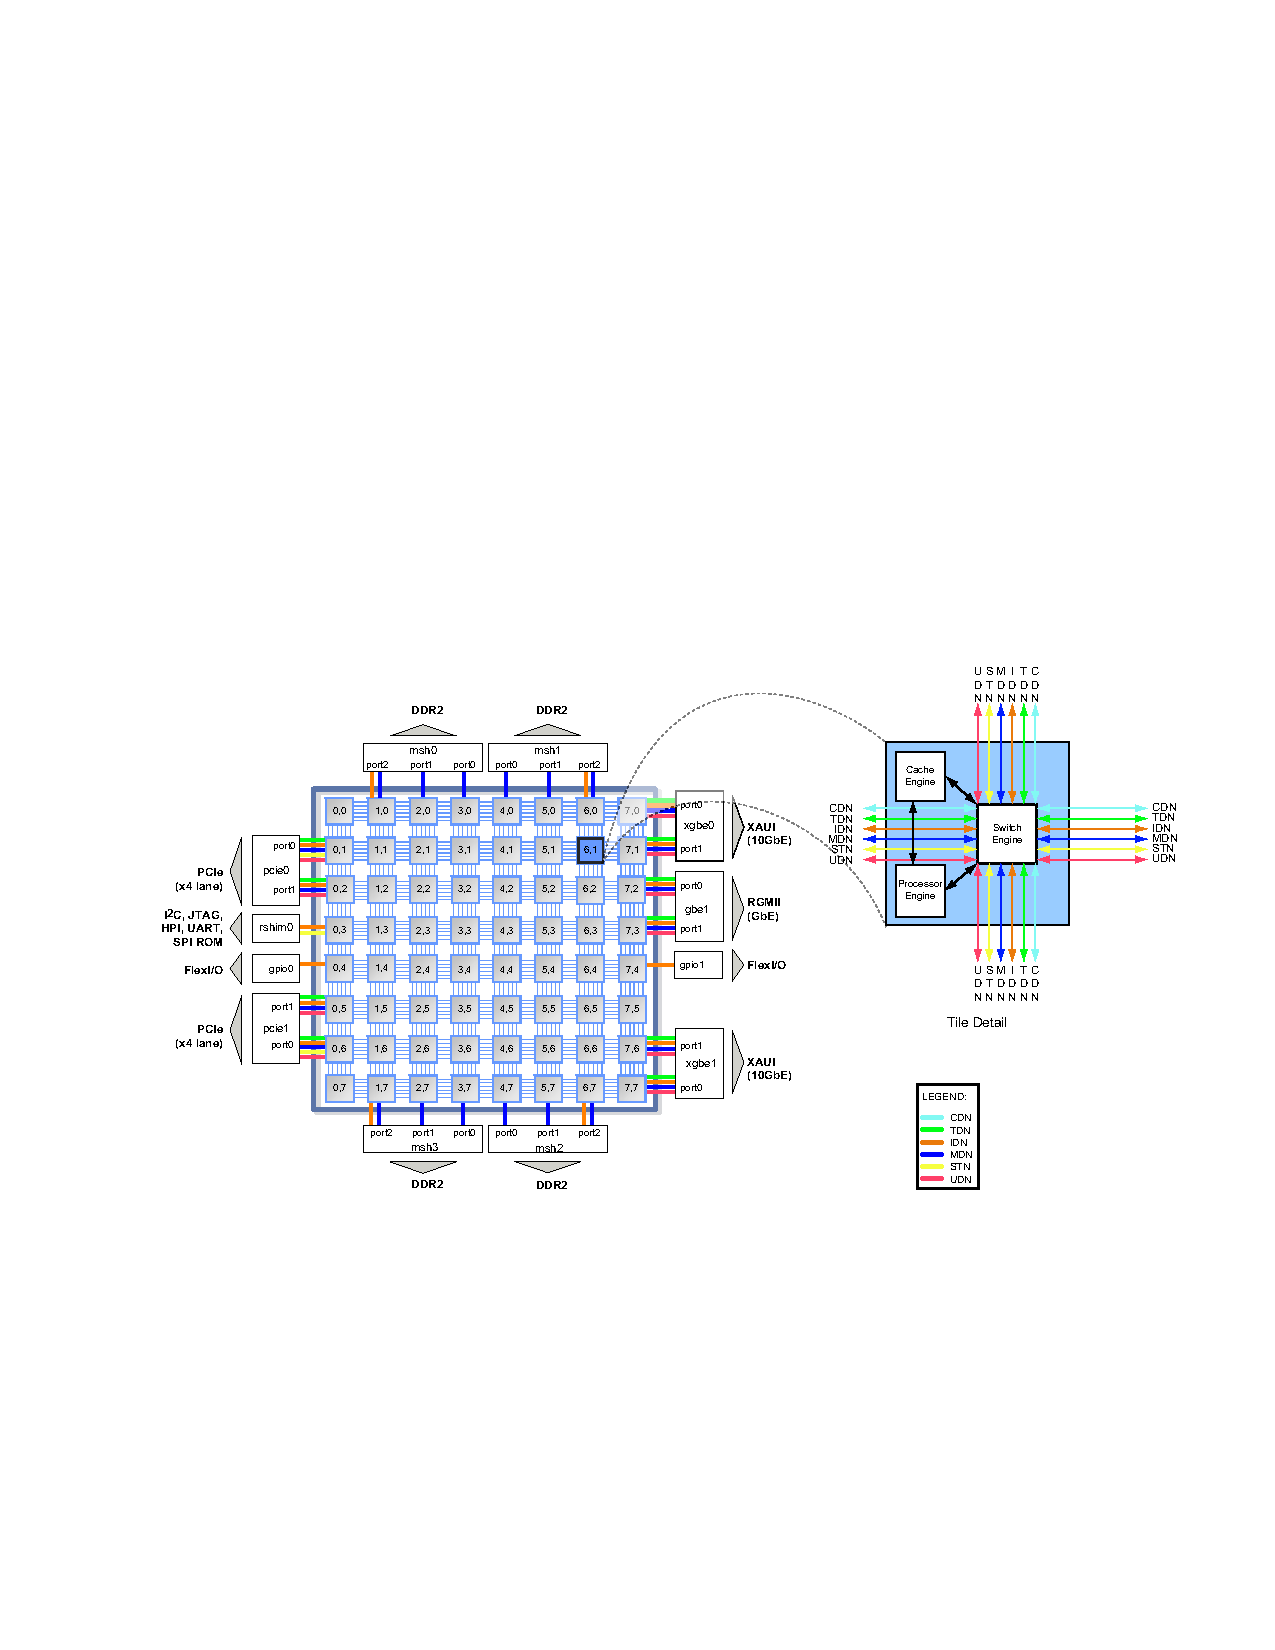
\includegraphics{TilePro64_schema.pdf}}
    \column{.5\textwidth} 
    \resizebox{\columnwidth}{!}{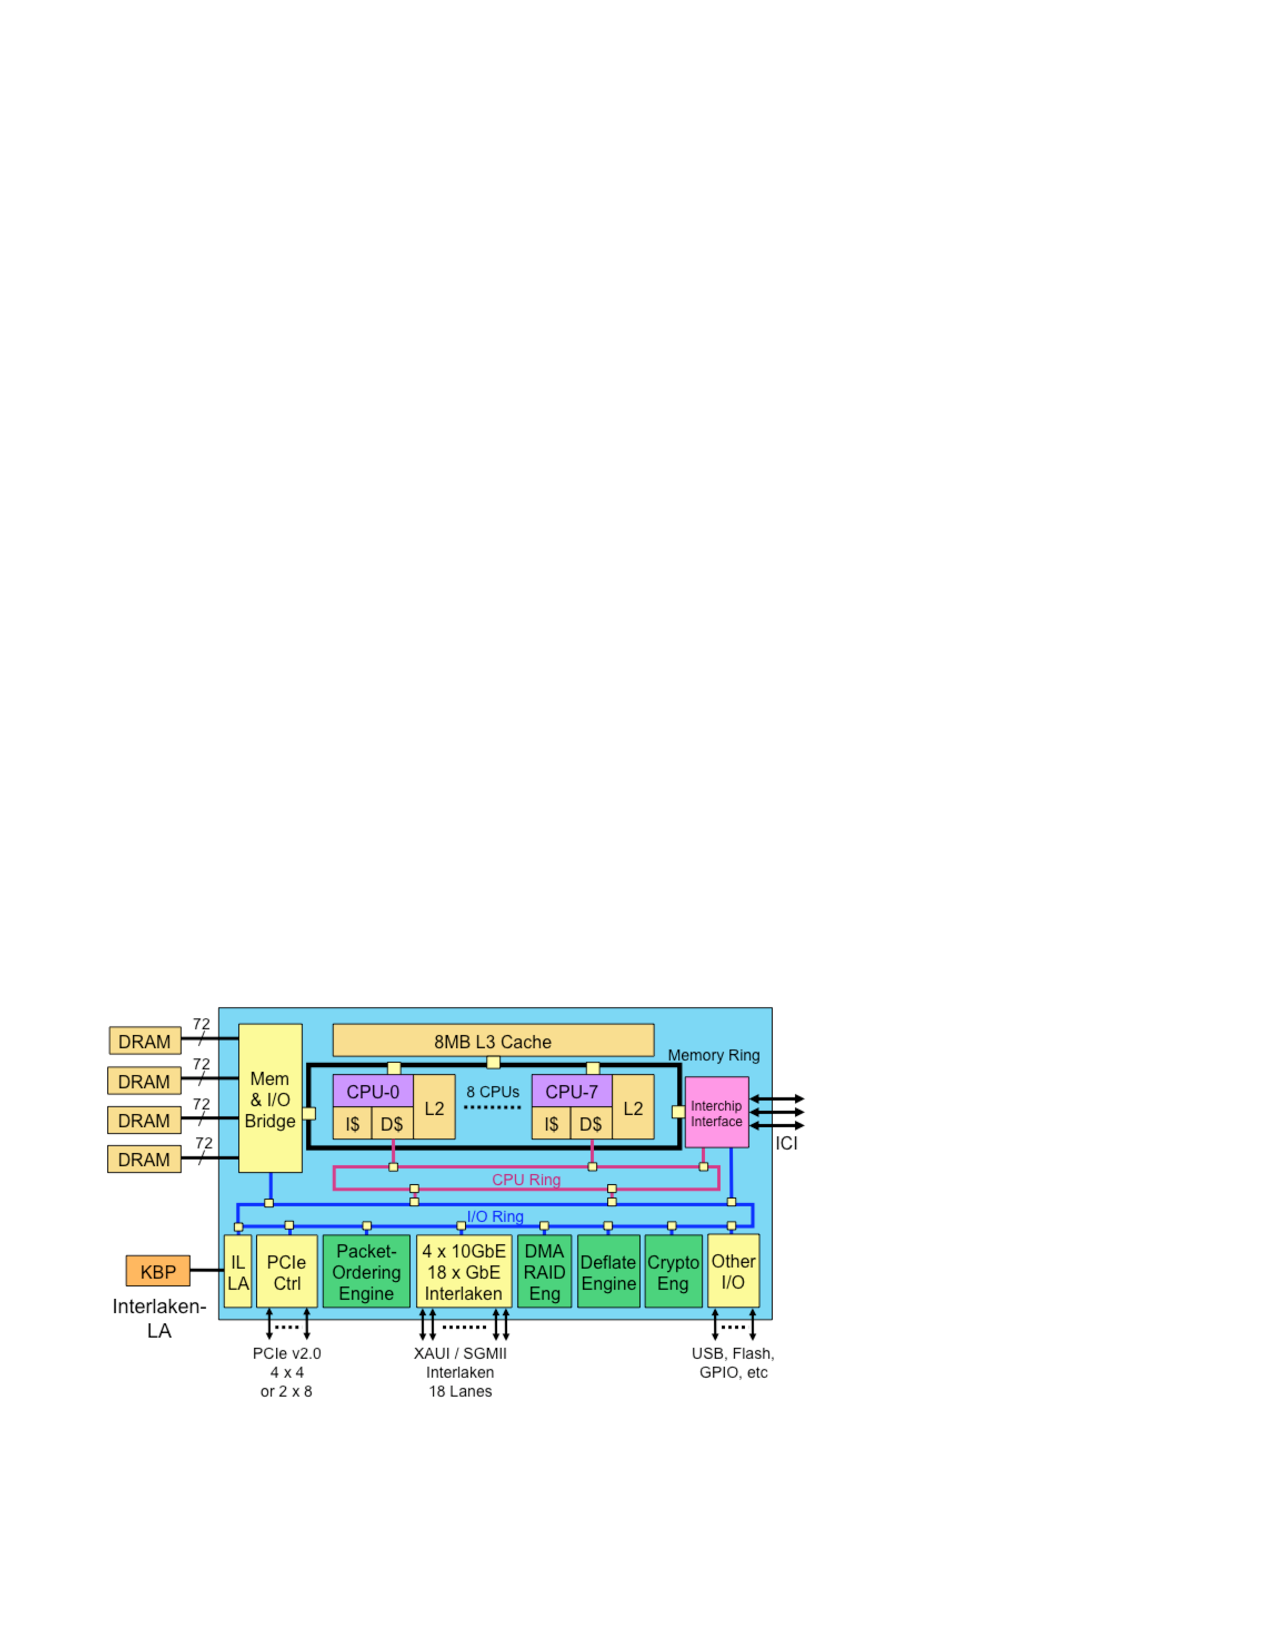
\includegraphics{NetLogic_schema.pdf}}
  \end{columns}
\end{frame}

\begin{frame}
  \frametitle{Reti di interconnessione del Tilera \tile}
  \begin{figure}
    \resizebox{\columnwidth}{!}{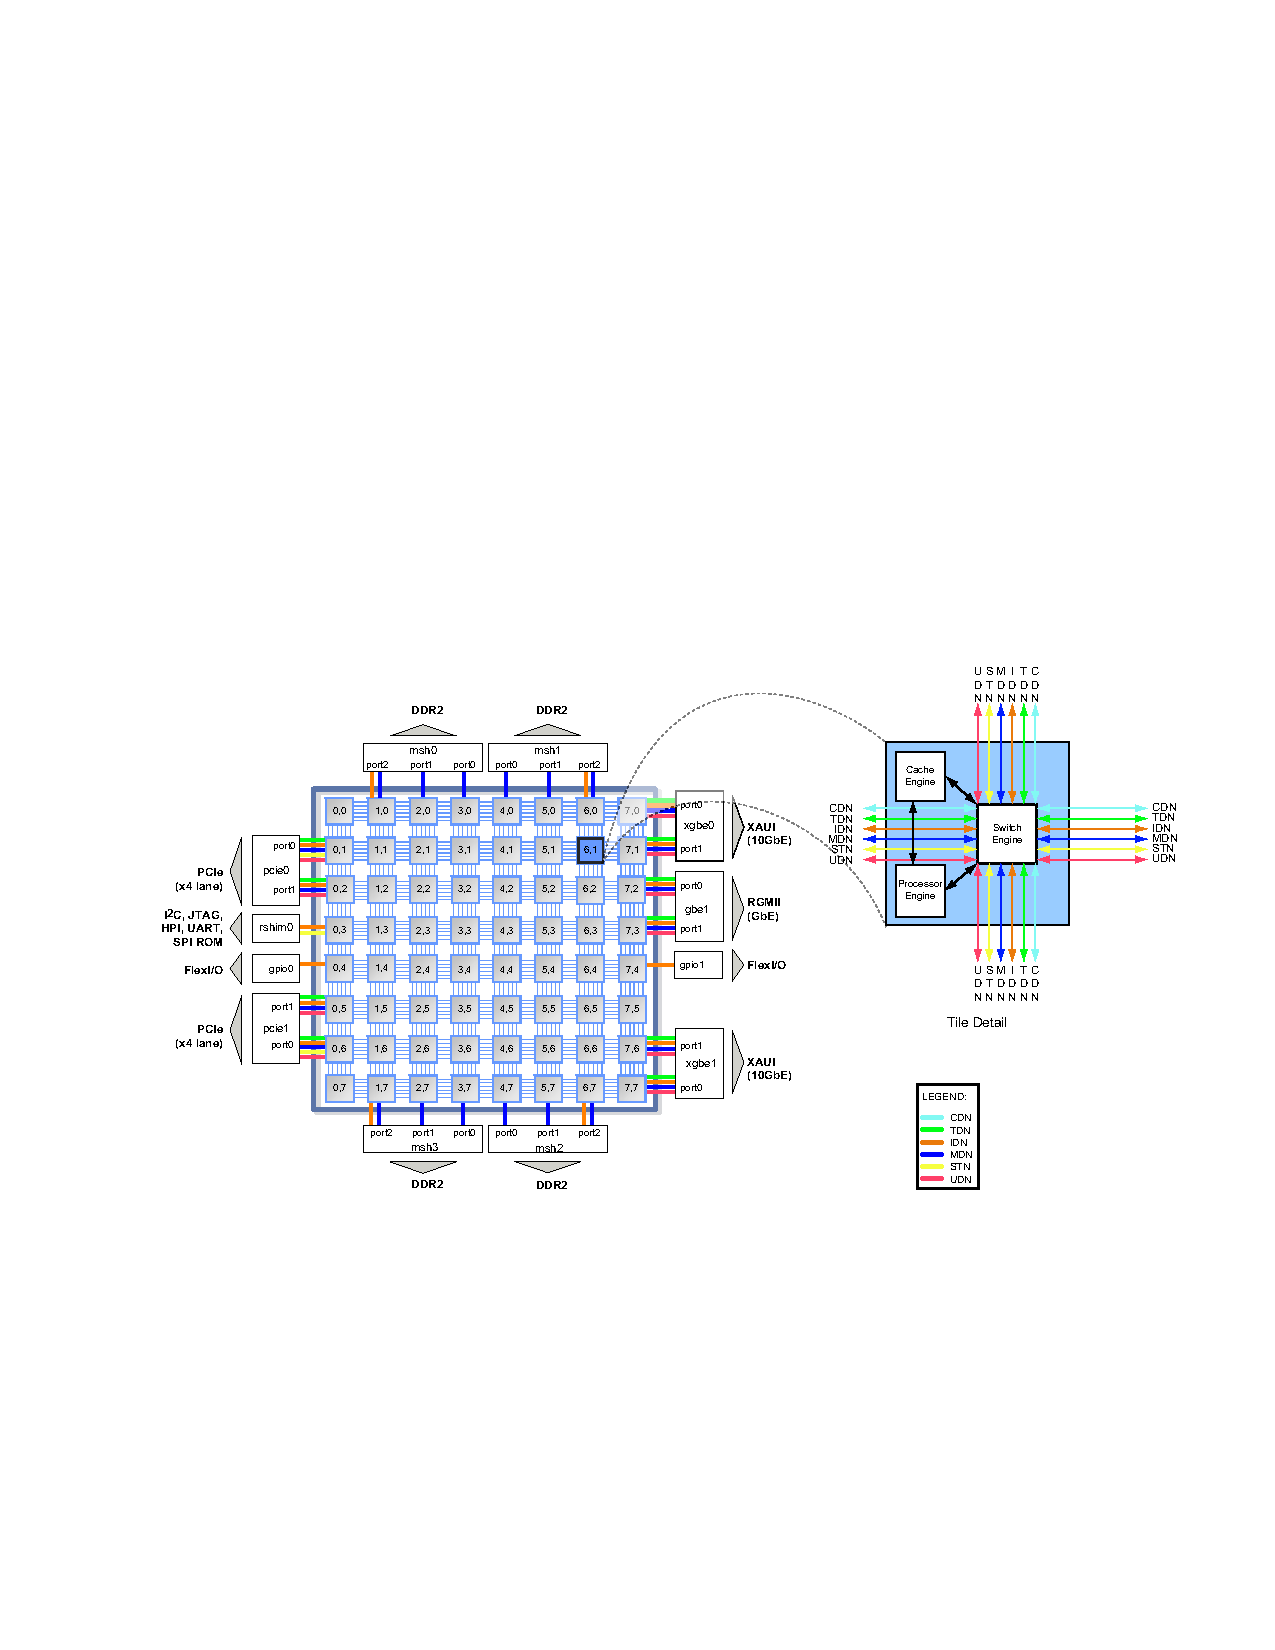
\includegraphics{TilePro64_schema.pdf}}
  \end{figure}
\end{frame}

\begin{frame}
  \frametitle{Dominio Applicativo}
   Computazioni con calcolo di grana fine:
    \begin{description}
    \item [Data Stream Processing] uno o pi\`u flussi contigui, rapidi e varianti nel tempo di dati; l'elaborazione sui dati in ingresso \`e fatta on-line:\hfill
      \begin{itemize}
      \item Monitoraggio e sicurezza di reti informatiche;
      \item Applicazioni finanziarie;
      \item Monitoraggio di sensori e Gestione delle emergenze;
      \item Altri \ldots
      \end{itemize}
    \item [Data Parallel] forma di parallelismo applicabile sia a computazioni su stream che su dato singolo; \`e caratterizzata dal partizionamento dei dati.
      \begin{itemize}
      \item le comunicazioni sono presenti nella realizzazione delle comunicazioni collettive e se esistono per le dipendenze sui dati (forme \emph{Stencil})
      \end{itemize}
    \end{description}
\end{frame}

\note{\scriptsize
  La diminuzione/minimizzazione della latenza di comunicazione \`e importante per applicazioni di grana fine che necessitano di supporti efficienti affinch\'e le prestazioni scalino con il numero di processi coinvolti. Domini applicativi a cui ci si rivolge sono in particolare:
  \begin{itemize}
  \item Data Stream Processing (DaSP);
  \item Implementazione di paradigmi di parallelismo Data Parallel, in particolare la forma Stencil.
  \end{itemize}
}

\begin{frame}
  \frametitle{Sulla grana del calcolo (1)}
  \begin{figure}
%    \resizebox{\columnwidth}{!}{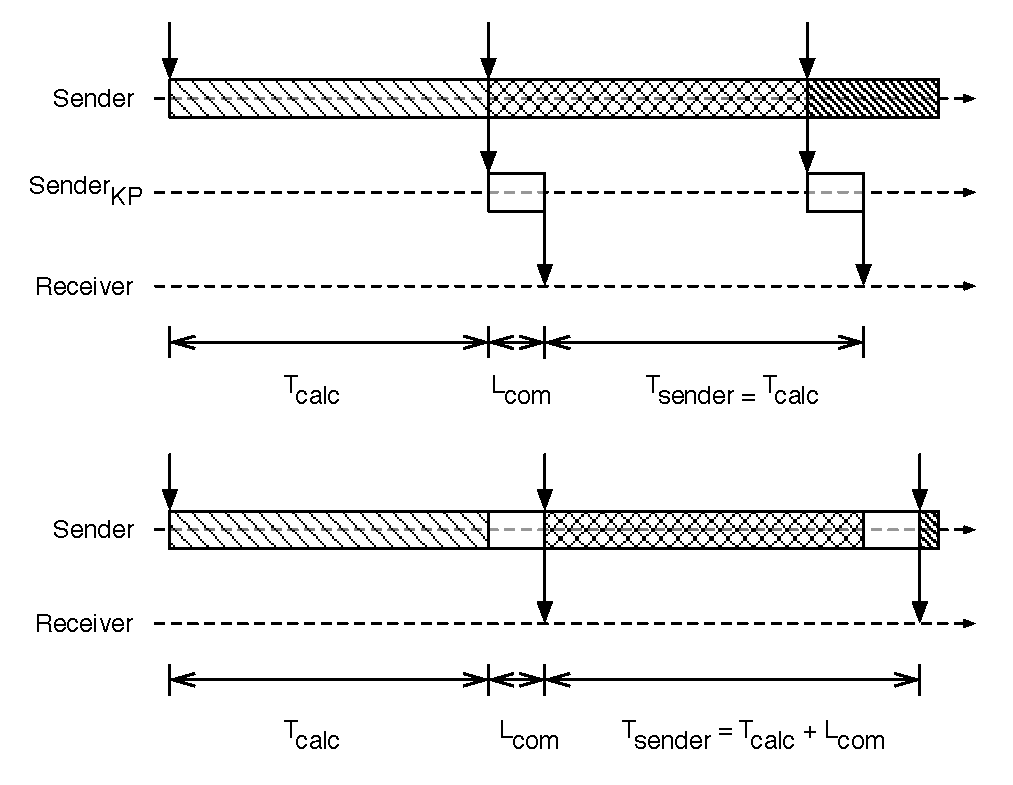
\includegraphics{servicetime_eg_coarse-grain.pdf}}
    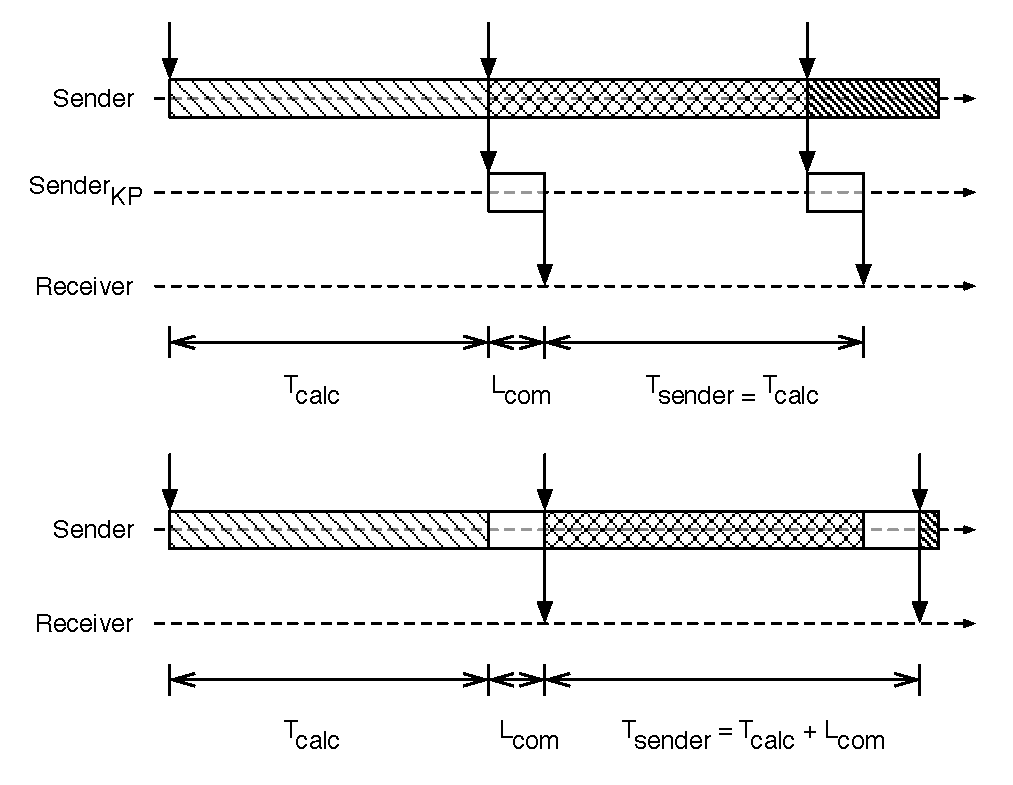
\includegraphics[height=2.7in]{servicetime_eg_coarse-grain.pdf}
  \end{figure}
\end{frame}

\note{\scriptsize A scopo esemplificativo si considera una parte di una applicazione su stream riguardante due moduli collegati in pipeline: si assume che il tempo di calcolo del primo modulo sia opportunamente dimensionato come il tempo di interarrivo dello stream. Se il tempo di calcolo \`e superiore di diversi ordini di grandezza alla latenza di comunicazione allora l'ottimizzazione della comunicazione (e.g. riduzione di qualche centinaio di cicli di clock della comunicazione) non consegue alcun vantaggio sul tempo di servizio effettivo del modulo: se \`e possibile la sovrapposizione del calcolo infatti la latenza di comunicazione \`e completamente mascherata dal tempo di calcolo, altrimenti la latenza di comunicazione si va a sommare al tempo di calcolo, risultando trascurabile. L'ottimizzazione delle prestazioni \`e invece apprezzabile quando la latenza di queste \`e dello stesso ordine di grandezza del tempo di calcolo.}

\begin{frame}
  \frametitle{Sulla grana del calcolo (2)}
  \begin{figure}
%    \resizebox{\pageheigth}{!}{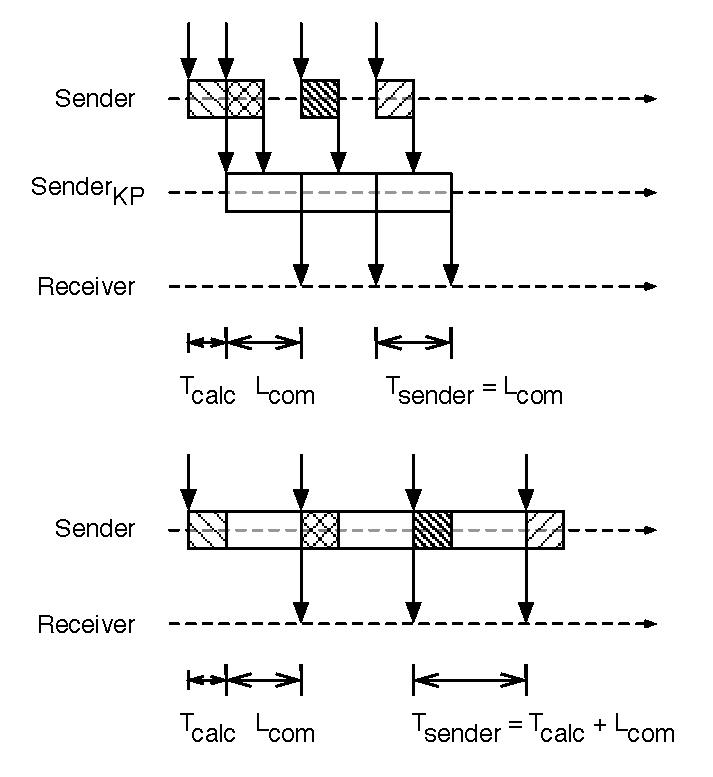
\includegraphics{servicetime_eg_fine-grain.pdf}}
    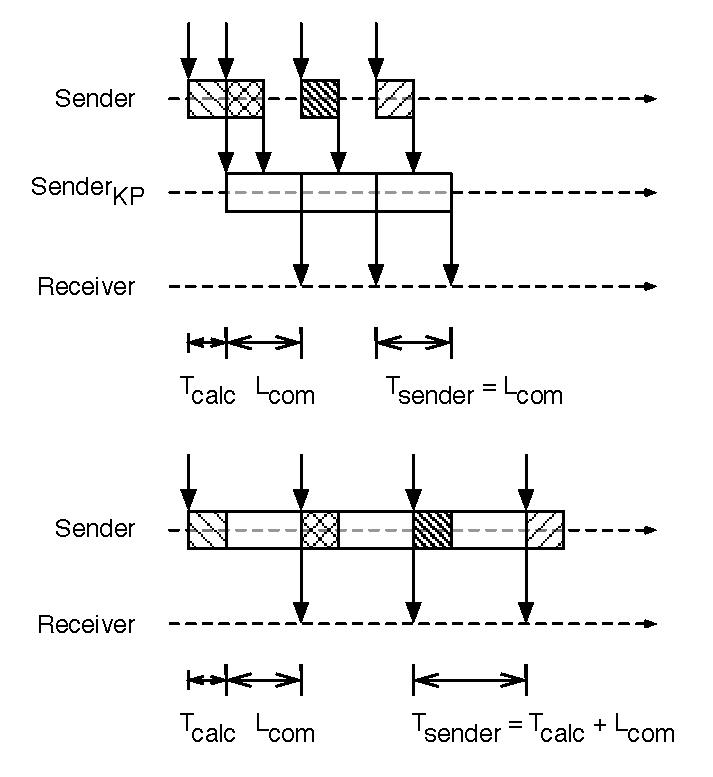
\includegraphics[height=2.7in]{servicetime_eg_fine-grain.pdf}
  \end{figure}
\end{frame}

\section{Supporto alle forme di comunicazione}

\begin{frame}
  \frametitle{Forme di comunicazione}
  \begin{columns}
    \column{.5\columnwidth}
    Canale simmetrico
    \column{.5\columnwidth}
    Canale asimmetrico in ingresso
  \end{columns}
  \begin{columns}
    \column{.5\columnwidth}
    \resizebox{\columnwidth}{!}{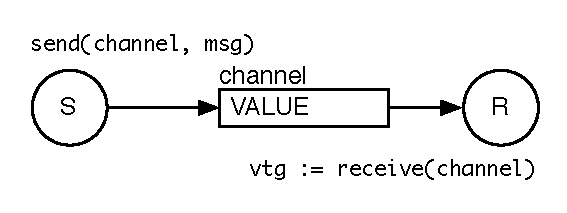
\includegraphics{abstract_sym.pdf}}
    \column{.5\columnwidth}
    \resizebox{\columnwidth}{!}{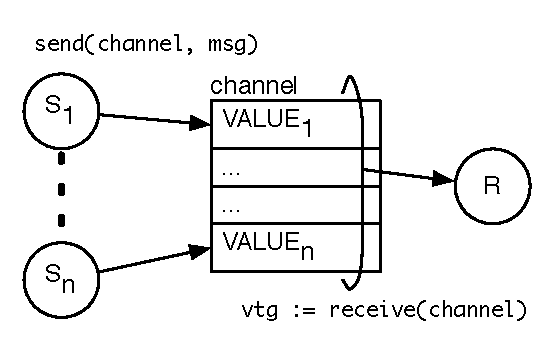
\includegraphics{abstract_asym.pdf}}
  \end{columns}
  \begin{itemize}
    \item Tipo 'riferimento'
    \item Grado di asincronia unitario
    \item Semantica Bloccante
    \item Protocollo Rdy-Ack
  \end{itemize}
\end{frame}

\begin{frame}[fragile]
  \frametitle{Implementazioni del canale simmetrico}
  \begin{description}
  \item [uso della Memoria Condivisa] \hfill
    \begin{itemize}
    \item \verb+ch_sym_sm_rdyack_no+ \hfill \\
      gestione predefinita della coerenza della cache;
    \item \verb+ch_sym_sm_rdyack+ \hfill \\
      configurazione della coerenza della cache che massimizza la localit\`a delle informazioni del supporto nei core consumatori;
    \item \verb+ch_sym_sm_nullack+ \hfill \\
      utilizzo di un diverso protocollo di comunicazione che garantisce la correttezza senza l'uso di istruzioni di barriera di memoria
    \end{itemize}
  \item [uso della UDN] \hfill
    \begin{itemize}
    \item \verb+ch_sym_udn+ \hfill \\
      corrispondenza biunivoca tra i canali firmware e i canali a livello processi
    \end{itemize}
  \end{description}
\end{frame}

\begin{frame}[fragile]
  \frametitle{Implementazioni del canale asimmetrico in ingresso}
  Un canale asimmetrico in ingresso pu\`o essere visto come un caso particolare di un certo numero di canali simmetrici in ingresso al processo destinatario, sui quali viene applicato non determinismo.
  \begin{description}
  \item [uso della Memoria Condivisa] \hfill
    \begin{itemize}
    \item \verb+ch_asymin_sm+ \hfill \\
      utilizzo del protocollo Rdy-Ack, con configurazione esplicita della coerenza della cache. Il destinatario implementa l'attesa con una lettura ciclica dei flag Rdy dei mittenti.
    \end{itemize}
  \item [uso della UDN] \hfill
    \begin{itemize}
    \item \verb+ch_asymin_udn+ \hfill \\
      uso di un unico canale firmware nel destinatario per la ricezione dei messaggi, uso di un canale firmware in ogni mittente per la ricezione dei segnali di Ack.
    \end{itemize}
  \end{description}
\end{frame}


\section{Esperimenti}

\subsection{Misura della Latenza di comunicazione}

\begin{frame}
  \frametitle{Misura della latenza di comunicazione}
  \begin{itemize}
  \item La latenza di comunicazione \`e misurata per mezzo di una applicazione ``ping-pong'':
    \begin{itemize}
    \item composta da due processi collegati da due canali,
    \item viene svolto lo scambio di $m$ messaggi tra i due processi;
    \end{itemize}
  \item La latenza di comunicazione \`e stimata con $\Lcom = \Tc / (2 \cdot m)$.
  \end{itemize}
  \begin{figure}
    \resizebox{\columnwidth}{!}{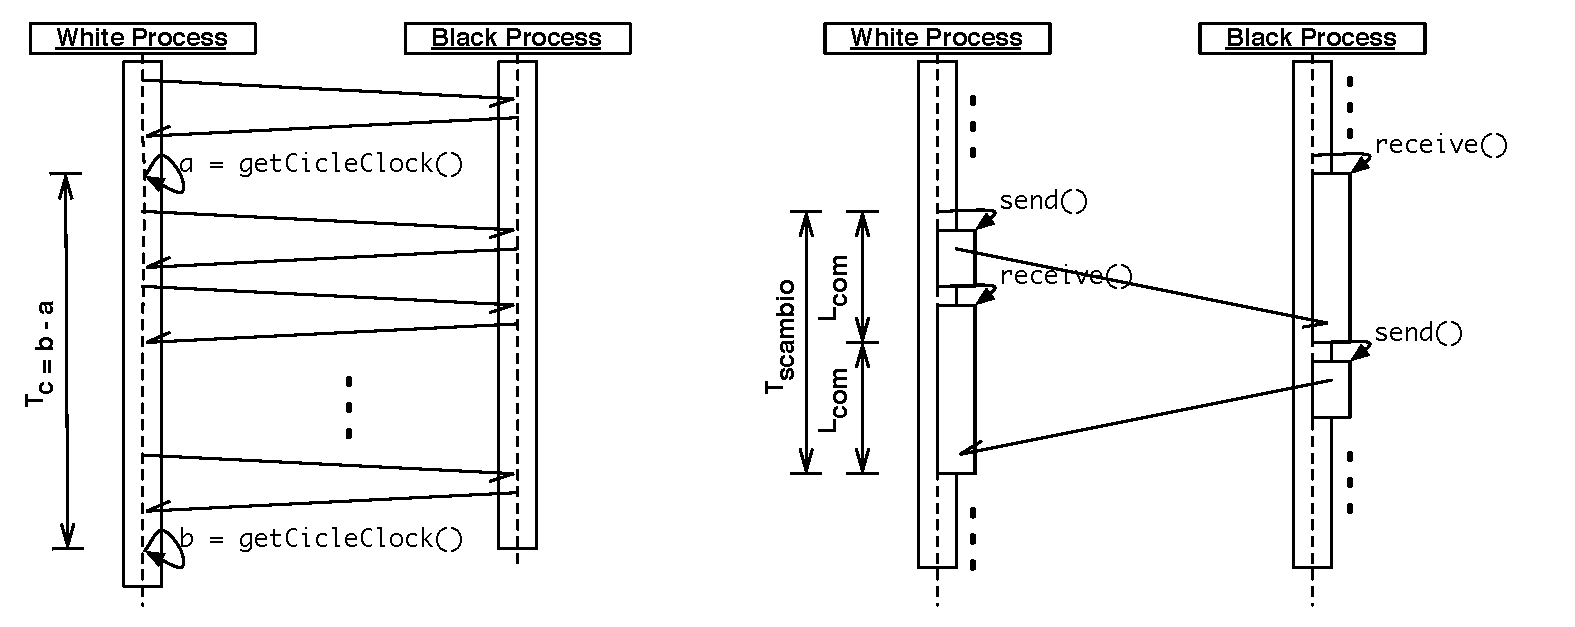
\includegraphics{schema_metering.pdf}}
  \end{figure}
\end{frame}

\begin{frame}
  \frametitle{Misura della latenza del canale simmetrico}
  \begin{figure}
    \resizebox{!}{2.7in}{% GNUPLOT: LaTeX picture with Postscript
\begingroup
  \makeatletter
  \providecommand\color[2][]{%
    \GenericError{(gnuplot) \space\space\space\@spaces}{%
      Package color not loaded in conjunction with
      terminal option `colourtext'%
    }{See the gnuplot documentation for explanation.%
    }{Either use 'blacktext' in gnuplot or load the package
      color.sty in LaTeX.}%
    \renewcommand\color[2][]{}%
  }%
  \providecommand\includegraphics[2][]{%
    \GenericError{(gnuplot) \space\space\space\@spaces}{%
      Package graphicx or graphics not loaded%
    }{See the gnuplot documentation for explanation.%
    }{The gnuplot epslatex terminal needs graphicx.sty or graphics.sty.}%
    \renewcommand\includegraphics[2][]{}%
  }%
  \providecommand\rotatebox[2]{#2}%
  \@ifundefined{ifGPcolor}{%
    \newif\ifGPcolor
    \GPcolortrue
  }{}%
  \@ifundefined{ifGPblacktext}{%
    \newif\ifGPblacktext
    \GPblacktexttrue
  }{}%
  % define a \g@addto@macro without @ in the name:
  \let\gplgaddtomacro\g@addto@macro
  % define empty templates for all commands taking text:
  \gdef\gplbacktext{}%
  \gdef\gplfronttext{}%
  \makeatother
  \ifGPblacktext
    % no textcolor at all
    \def\colorrgb#1{}%
    \def\colorgray#1{}%
  \else
    % gray or color?
    \ifGPcolor
      \def\colorrgb#1{\color[rgb]{#1}}%
      \def\colorgray#1{\color[gray]{#1}}%
      \expandafter\def\csname LTw\endcsname{\color{white}}%
      \expandafter\def\csname LTb\endcsname{\color{black}}%
      \expandafter\def\csname LTa\endcsname{\color{black}}%
      \expandafter\def\csname LT0\endcsname{\color[rgb]{1,0,0}}%
      \expandafter\def\csname LT1\endcsname{\color[rgb]{0,1,0}}%
      \expandafter\def\csname LT2\endcsname{\color[rgb]{0,0,1}}%
      \expandafter\def\csname LT3\endcsname{\color[rgb]{1,0,1}}%
      \expandafter\def\csname LT4\endcsname{\color[rgb]{0,1,1}}%
      \expandafter\def\csname LT5\endcsname{\color[rgb]{1,1,0}}%
      \expandafter\def\csname LT6\endcsname{\color[rgb]{0,0,0}}%
      \expandafter\def\csname LT7\endcsname{\color[rgb]{1,0.3,0}}%
      \expandafter\def\csname LT8\endcsname{\color[rgb]{0.5,0.5,0.5}}%
    \else
      % gray
      \def\colorrgb#1{\color{black}}%
      \def\colorgray#1{\color[gray]{#1}}%
      \expandafter\def\csname LTw\endcsname{\color{white}}%
      \expandafter\def\csname LTb\endcsname{\color{black}}%
      \expandafter\def\csname LTa\endcsname{\color{black}}%
      \expandafter\def\csname LT0\endcsname{\color{black}}%
      \expandafter\def\csname LT1\endcsname{\color{black}}%
      \expandafter\def\csname LT2\endcsname{\color{black}}%
      \expandafter\def\csname LT3\endcsname{\color{black}}%
      \expandafter\def\csname LT4\endcsname{\color{black}}%
      \expandafter\def\csname LT5\endcsname{\color{black}}%
      \expandafter\def\csname LT6\endcsname{\color{black}}%
      \expandafter\def\csname LT7\endcsname{\color{black}}%
      \expandafter\def\csname LT8\endcsname{\color{black}}%
    \fi
  \fi
  \setlength{\unitlength}{0.0500bp}%
  \begin{picture}(7200.00,5040.00)%
    \gplgaddtomacro\gplbacktext{%
      \csname LTb\endcsname%
      \put(946,704){\makebox(0,0)[r]{\strut{} 0}}%
      \put(946,1128){\makebox(0,0)[r]{\strut{} 50}}%
      \put(946,1553){\makebox(0,0)[r]{\strut{} 100}}%
      \put(946,1977){\makebox(0,0)[r]{\strut{} 150}}%
      \put(946,2402){\makebox(0,0)[r]{\strut{} 200}}%
      \put(946,2826){\makebox(0,0)[r]{\strut{} 250}}%
      \put(946,3251){\makebox(0,0)[r]{\strut{} 300}}%
      \put(946,3675){\makebox(0,0)[r]{\strut{} 350}}%
      \put(2223,484){\makebox(0,0){\strut{}1}}%
      \put(3369,484){\makebox(0,0){\strut{}8}}%
      \put(4514,484){\makebox(0,0){\strut{}14}}%
      \put(5791,704){\makebox(0,0)[l]{\strut{} 0}}%
      \put(5791,1071){\makebox(0,0)[l]{\strut{} 0.05}}%
      \put(5791,1438){\makebox(0,0)[l]{\strut{} 0.1}}%
      \put(5791,1805){\makebox(0,0)[l]{\strut{} 0.15}}%
      \put(5791,2172){\makebox(0,0)[l]{\strut{} 0.2}}%
      \put(5791,2539){\makebox(0,0)[l]{\strut{} 0.25}}%
      \put(5791,2906){\makebox(0,0)[l]{\strut{} 0.3}}%
      \put(5791,3273){\makebox(0,0)[l]{\strut{} 0.35}}%
      \put(5791,3640){\makebox(0,0)[l]{\strut{} 0.4}}%
      \put(176,2189){\rotatebox{-270}{\makebox(0,0){\strut{}$\mathrm{L}_{\mathrm{com}} \; (\,\tau\,)$}}}%
      \put(6692,2189){\rotatebox{-270}{\makebox(0,0){\strut{}$\mathrm{L}_{\mathrm{com}} \; (\,\mu\mathrm{sec}\,)$}}}%
      \put(3368,154){\makebox(0,0){\strut{}number of hops}}%
    }%
    \gplgaddtomacro\gplfronttext{%
      \csname LTb\endcsname%
      \put(4804,4867){\makebox(0,0)[r]{\strut{}uso della Rete di Interconnessione}}%
      \csname LTb\endcsname%
      \put(4804,4647){\makebox(0,0)[r]{\strut{}uso della Memoria Condivisa, coerenza cache predefinita}}%
      \csname LTb\endcsname%
      \put(4804,4427){\makebox(0,0)[r]{\strut{}uso della SM, configurazione coerenza cache}}%
      \csname LTb\endcsname%
      \put(4804,4207){\makebox(0,0)[r]{\strut{}uso della Memoria Condivisa, non uso di memory barrier}}%
    }%
    \gplbacktext
    \put(0,0){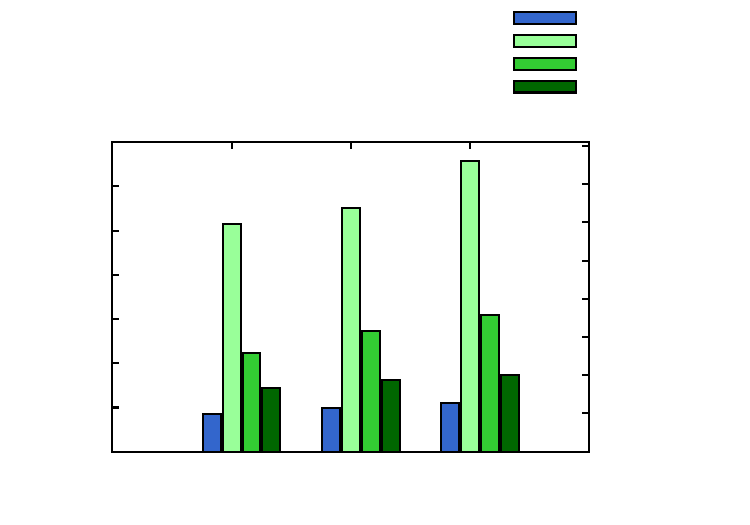
\includegraphics{2_5_sym_all_color}}%
    \gplfronttext
  \end{picture}%
\endgroup
}
  \end{figure}
\end{frame}

\begin{frame}
  \frametitle{Misura della latenza del canale asimmetrico}
  \begin{figure}
    \resizebox{!}{2.7in}{% GNUPLOT: LaTeX picture with Postscript
\begingroup
  \makeatletter
  \providecommand\color[2][]{%
    \GenericError{(gnuplot) \space\space\space\@spaces}{%
      Package color not loaded in conjunction with
      terminal option `colourtext'%
    }{See the gnuplot documentation for explanation.%
    }{Either use 'blacktext' in gnuplot or load the package
      color.sty in LaTeX.}%
    \renewcommand\color[2][]{}%
  }%
  \providecommand\includegraphics[2][]{%
    \GenericError{(gnuplot) \space\space\space\@spaces}{%
      Package graphicx or graphics not loaded%
    }{See the gnuplot documentation for explanation.%
    }{The gnuplot epslatex terminal needs graphicx.sty or graphics.sty.}%
    \renewcommand\includegraphics[2][]{}%
  }%
  \providecommand\rotatebox[2]{#2}%
  \@ifundefined{ifGPcolor}{%
    \newif\ifGPcolor
    \GPcolortrue
  }{}%
  \@ifundefined{ifGPblacktext}{%
    \newif\ifGPblacktext
    \GPblacktexttrue
  }{}%
  % define a \g@addto@macro without @ in the name:
  \let\gplgaddtomacro\g@addto@macro
  % define empty templates for all commands taking text:
  \gdef\gplbacktext{}%
  \gdef\gplfronttext{}%
  \makeatother
  \ifGPblacktext
    % no textcolor at all
    \def\colorrgb#1{}%
    \def\colorgray#1{}%
  \else
    % gray or color?
    \ifGPcolor
      \def\colorrgb#1{\color[rgb]{#1}}%
      \def\colorgray#1{\color[gray]{#1}}%
      \expandafter\def\csname LTw\endcsname{\color{white}}%
      \expandafter\def\csname LTb\endcsname{\color{black}}%
      \expandafter\def\csname LTa\endcsname{\color{black}}%
      \expandafter\def\csname LT0\endcsname{\color[rgb]{1,0,0}}%
      \expandafter\def\csname LT1\endcsname{\color[rgb]{0,1,0}}%
      \expandafter\def\csname LT2\endcsname{\color[rgb]{0,0,1}}%
      \expandafter\def\csname LT3\endcsname{\color[rgb]{1,0,1}}%
      \expandafter\def\csname LT4\endcsname{\color[rgb]{0,1,1}}%
      \expandafter\def\csname LT5\endcsname{\color[rgb]{1,1,0}}%
      \expandafter\def\csname LT6\endcsname{\color[rgb]{0,0,0}}%
      \expandafter\def\csname LT7\endcsname{\color[rgb]{1,0.3,0}}%
      \expandafter\def\csname LT8\endcsname{\color[rgb]{0.5,0.5,0.5}}%
    \else
      % gray
      \def\colorrgb#1{\color{black}}%
      \def\colorgray#1{\color[gray]{#1}}%
      \expandafter\def\csname LTw\endcsname{\color{white}}%
      \expandafter\def\csname LTb\endcsname{\color{black}}%
      \expandafter\def\csname LTa\endcsname{\color{black}}%
      \expandafter\def\csname LT0\endcsname{\color{black}}%
      \expandafter\def\csname LT1\endcsname{\color{black}}%
      \expandafter\def\csname LT2\endcsname{\color{black}}%
      \expandafter\def\csname LT3\endcsname{\color{black}}%
      \expandafter\def\csname LT4\endcsname{\color{black}}%
      \expandafter\def\csname LT5\endcsname{\color{black}}%
      \expandafter\def\csname LT6\endcsname{\color{black}}%
      \expandafter\def\csname LT7\endcsname{\color{black}}%
      \expandafter\def\csname LT8\endcsname{\color{black}}%
    \fi
  \fi
  \setlength{\unitlength}{0.0500bp}%
  \begin{picture}(7200.00,5040.00)%
    \gplgaddtomacro\gplbacktext{%
      \csname LTb\endcsname%
      \put(946,704){\makebox(0,0)[r]{\strut{} 0}}%
      \put(946,1059){\makebox(0,0)[r]{\strut{} 50}}%
      \put(946,1413){\makebox(0,0)[r]{\strut{} 100}}%
      \put(946,1768){\makebox(0,0)[r]{\strut{} 150}}%
      \put(946,2122){\makebox(0,0)[r]{\strut{} 200}}%
      \put(946,2477){\makebox(0,0)[r]{\strut{} 250}}%
      \put(946,2831){\makebox(0,0)[r]{\strut{} 300}}%
      \put(946,3186){\makebox(0,0)[r]{\strut{} 350}}%
      \put(946,3540){\makebox(0,0)[r]{\strut{} 400}}%
      \put(946,3895){\makebox(0,0)[r]{\strut{} 450}}%
      \put(2256,484){\makebox(0,0){\strut{}1}}%
      \put(3435,484){\makebox(0,0){\strut{}8}}%
      \put(4613,484){\makebox(0,0){\strut{}14}}%
      \put(5923,704){\makebox(0,0)[l]{\strut{} 0}}%
      \put(5923,1317){\makebox(0,0)[l]{\strut{} 0.1}}%
      \put(5923,1930){\makebox(0,0)[l]{\strut{} 0.2}}%
      \put(5923,2543){\makebox(0,0)[l]{\strut{} 0.3}}%
      \put(5923,3156){\makebox(0,0)[l]{\strut{} 0.4}}%
      \put(5923,3769){\makebox(0,0)[l]{\strut{} 0.5}}%
      \put(176,2299){\rotatebox{-270}{\makebox(0,0){\strut{}$\mathrm{L}_{\mathrm{com}} \; (\,\tau\,)$}}}%
      \put(6692,2299){\rotatebox{-270}{\makebox(0,0){\strut{}$\mathrm{L}_{\mathrm{com}} \; (\,\mu\mathrm{sec}\,)$}}}%
      \put(3434,154){\makebox(0,0){\strut{}number of hops}}%
    }%
    \gplgaddtomacro\gplfronttext{%
      \csname LTb\endcsname%
      \put(4936,4867){\makebox(0,0)[r]{\strut{}uso della Rete di Interconnessione}}%
      \csname LTb\endcsname%
      \put(4936,4647){\makebox(0,0)[r]{\strut{}uso della memoria condivisa, allocati tutti i mittenti}}%
      \csname LTb\endcsname%
      \put(4936,4427){\makebox(0,0)[r]{\strut{}uso della memoria condivisa, allocato un unico mittente}}%
    }%
    \gplbacktext
    \put(0,0){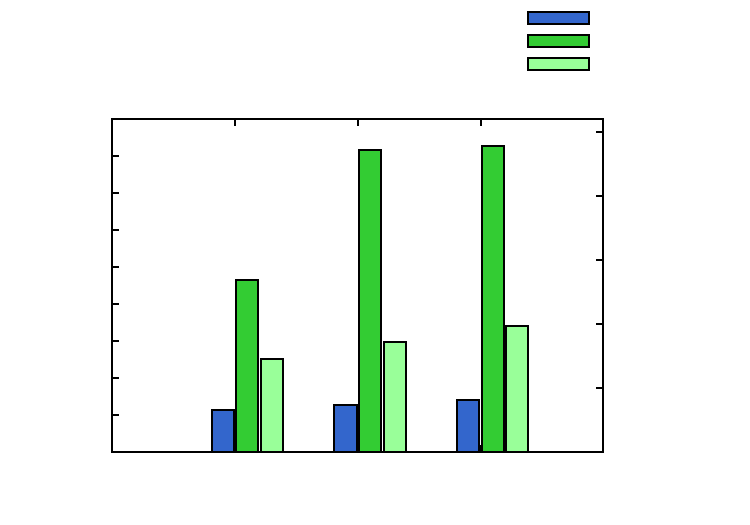
\includegraphics{2_5_asymin_all_color}}%
    \gplfronttext
  \end{picture}%
\endgroup
}
  \end{figure}
\end{frame}

\subsection{Benchmark}

\begin{frame}
  \frametitle{Benchmark: prodotto matrice-vettore su stream}
  \begin{flalign*}
  \mathbf{A} &= (a_{ij})_{i=1,\ldots,\mathrm{M}, \, j=1,\ldots,\mathrm{M}} \in \mathbb{Z}^{\mathrm{MxM}} \\
  \mathbf{b} &= (b_1,\ldots,b_\mathrm{M}) \in \mathbb{Z}^{\mathrm{M}} \\
  \mathbf{c} &= (c_1,\ldots,c_\mathrm{M}) = \mathbf{A} \cdot \mathbf{b} \in \mathbb{Z}^{\mathrm{M}} \\
  &\forall \; i \in \{1,\ldots,\mathrm{M}\} \; : \; c_i = \mathbf{a}_i \cdot \mathbf{b} = \sum_{j=1}^{\mathrm{M}} a_{ij} \cdot b_j 
  \end{flalign*}
  %% \[ \mathbf{A} = (a_{ij})_{i=1,\ldots,\mathrm{M}, \, j=1,\ldots,\mathrm{M}} \in \mathbb{Z}^{\mathrm{MxM}} \]
  %% \[ \mathbf{b} = (b_1,\ldots,b_\mathrm{M}) \in \mathbb{Z}^{\mathrm{M}} \]
  %% \[ \mathbf{c} = (c_1,\ldots,c_\mathrm{M}) = \mathbf{A} \cdot \mathbf{b} \in \mathbb{Z}^{\mathrm{M}} \]
  %% \[ \forall \; i \in \{1,\ldots,\mathrm{M}\} \; : \; c_i = \mathbf{a}_i \cdot \mathbf{b} = \sum_{j=1}^{\mathrm{M}} a_{ij} \cdot b_j  \]
  \begin{columns}[c]
    \column{.5\textwidth}
    \begin{figure}
      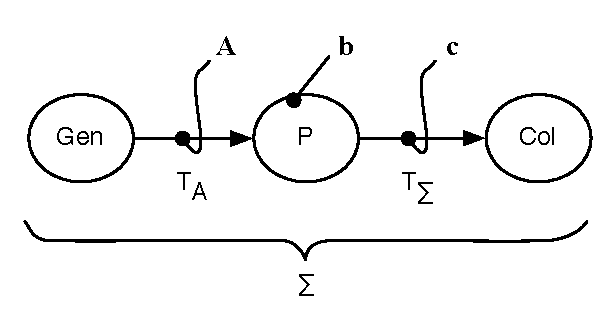
\includegraphics[scale=.5]{grafo_sigma_compatto_slide.pdf}
    \end{figure}  
    \column{.5\textwidth}
    \begin{itemize}
    \item computazione su stream di matrici
    \item il vettore $\mathbf{b}$ \`e costante per tutta l'esecuzione
    \end{itemize}
  \end{columns}
  
\end{frame}


\note{Si basa sul partizionamento dei dati in ingresso e sulla replicazione della funzione di calcolo nelle unit\`a worker.}

\begin{frame}
  \frametitle{Benchmark: soluzione parallela}
  \begin{columns}[c]
    \column{.5\textwidth}
    \begin{itemize}
\item Data Parallel Map
  \begin{itemize}
  \item partizionamento di una matrice per righe
  \item replicazione del vettore $\mathbf{b}$ nei processi worker
  \end{itemize}
\item Multicast strutturata ad albero distribuito nei worker
\item $\inTsubsystemId = \; 2 \cdot \inTsymsend + \inTcalc / n + \inTasyminsend$
\end{itemize}
    \column{.5\textwidth} 
  \begin{figure}
    \resizebox{!}{\linewidth}{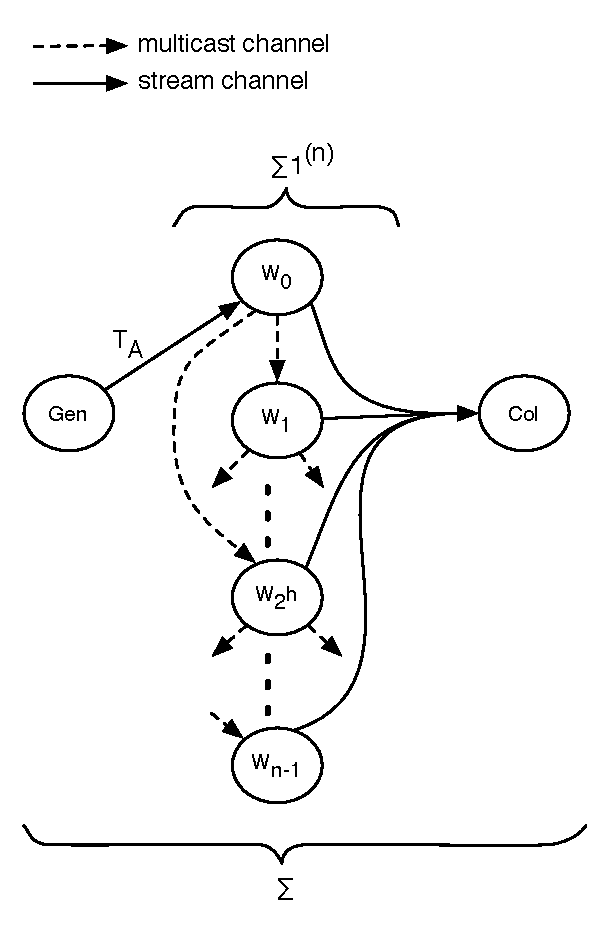
\includegraphics{grafo_sigma_vert.pdf}}
  \end{figure}  

  \end{columns}
\end{frame}

\begin{frame}
  \frametitle{Confronto: tempo di servizio (1)}
  \begin{itemize}
  \item Tempo di interarrivo 4.627 \musec
  \item Dimensione delle matrici 56x56
  \item Tempo di servizio migliore UDN 6.177 \musec
  \item Tempo di servizio migliore SM 8.735 \musec
  \end{itemize}
  \begin{columns}
    \column{.5\columnwidth}
    \resizebox{\columnwidth}{!}{% GNUPLOT: LaTeX picture with Postscript
\begingroup
  \makeatletter
  \providecommand\color[2][]{%
    \GenericError{(gnuplot) \space\space\space\@spaces}{%
      Package color not loaded in conjunction with
      terminal option `colourtext'%
    }{See the gnuplot documentation for explanation.%
    }{Either use 'blacktext' in gnuplot or load the package
      color.sty in LaTeX.}%
    \renewcommand\color[2][]{}%
  }%
  \providecommand\includegraphics[2][]{%
    \GenericError{(gnuplot) \space\space\space\@spaces}{%
      Package graphicx or graphics not loaded%
    }{See the gnuplot documentation for explanation.%
    }{The gnuplot epslatex terminal needs graphicx.sty or graphics.sty.}%
    \renewcommand\includegraphics[2][]{}%
  }%
  \providecommand\rotatebox[2]{#2}%
  \@ifundefined{ifGPcolor}{%
    \newif\ifGPcolor
    \GPcolortrue
  }{}%
  \@ifundefined{ifGPblacktext}{%
    \newif\ifGPblacktext
    \GPblacktexttrue
  }{}%
  % define a \g@addto@macro without @ in the name:
  \let\gplgaddtomacro\g@addto@macro
  % define empty templates for all commands taking text:
  \gdef\gplbacktext{}%
  \gdef\gplfronttext{}%
  \makeatother
  \ifGPblacktext
    % no textcolor at all
    \def\colorrgb#1{}%
    \def\colorgray#1{}%
  \else
    % gray or color?
    \ifGPcolor
      \def\colorrgb#1{\color[rgb]{#1}}%
      \def\colorgray#1{\color[gray]{#1}}%
      \expandafter\def\csname LTw\endcsname{\color{white}}%
      \expandafter\def\csname LTb\endcsname{\color{black}}%
      \expandafter\def\csname LTa\endcsname{\color{black}}%
      \expandafter\def\csname LT0\endcsname{\color[rgb]{1,0,0}}%
      \expandafter\def\csname LT1\endcsname{\color[rgb]{0,1,0}}%
      \expandafter\def\csname LT2\endcsname{\color[rgb]{0,0,1}}%
      \expandafter\def\csname LT3\endcsname{\color[rgb]{1,0,1}}%
      \expandafter\def\csname LT4\endcsname{\color[rgb]{0,1,1}}%
      \expandafter\def\csname LT5\endcsname{\color[rgb]{1,1,0}}%
      \expandafter\def\csname LT6\endcsname{\color[rgb]{0,0,0}}%
      \expandafter\def\csname LT7\endcsname{\color[rgb]{1,0.3,0}}%
      \expandafter\def\csname LT8\endcsname{\color[rgb]{0.5,0.5,0.5}}%
    \else
      % gray
      \def\colorrgb#1{\color{black}}%
      \def\colorgray#1{\color[gray]{#1}}%
      \expandafter\def\csname LTw\endcsname{\color{white}}%
      \expandafter\def\csname LTb\endcsname{\color{black}}%
      \expandafter\def\csname LTa\endcsname{\color{black}}%
      \expandafter\def\csname LT0\endcsname{\color{black}}%
      \expandafter\def\csname LT1\endcsname{\color{black}}%
      \expandafter\def\csname LT2\endcsname{\color{black}}%
      \expandafter\def\csname LT3\endcsname{\color{black}}%
      \expandafter\def\csname LT4\endcsname{\color{black}}%
      \expandafter\def\csname LT5\endcsname{\color{black}}%
      \expandafter\def\csname LT6\endcsname{\color{black}}%
      \expandafter\def\csname LT7\endcsname{\color{black}}%
      \expandafter\def\csname LT8\endcsname{\color{black}}%
    \fi
  \fi
  \setlength{\unitlength}{0.0500bp}%
  \begin{picture}(7200.00,5040.00)%
    \gplgaddtomacro\gplbacktext{%
      \csname LTb\endcsname%
      \put(814,1325){\makebox(0,0)[r]{\strut{} 10}}%
      \csname LTb\endcsname%
      \put(814,2015){\makebox(0,0)[r]{\strut{} 20}}%
      \csname LTb\endcsname%
      \put(814,2705){\makebox(0,0)[r]{\strut{} 30}}%
      \csname LTb\endcsname%
      \put(814,3395){\makebox(0,0)[r]{\strut{} 40}}%
      \csname LTb\endcsname%
      \put(814,4085){\makebox(0,0)[r]{\strut{} 50}}%
      \csname LTb\endcsname%
      \put(814,4775){\makebox(0,0)[r]{\strut{} 60}}%
      \csname LTb\endcsname%
      \put(1839,484){\makebox(0,0){\strut{} 10}}%
      \csname LTb\endcsname%
      \put(2832,484){\makebox(0,0){\strut{} 20}}%
      \csname LTb\endcsname%
      \put(3825,484){\makebox(0,0){\strut{} 30}}%
      \csname LTb\endcsname%
      \put(4818,484){\makebox(0,0){\strut{} 40}}%
      \csname LTb\endcsname%
      \put(5810,484){\makebox(0,0){\strut{} 50}}%
      \csname LTb\endcsname%
      \put(6803,484){\makebox(0,0){\strut{} 60}}%
      \put(176,2739){\rotatebox{-270}{\makebox(0,0){\strut{}scalability}}}%
      \put(3874,154){\makebox(0,0){\strut{}$n$ parallel degree}}%
    }%
    \gplgaddtomacro\gplfronttext{%
      \csname LTb\endcsname%
      \put(3322,4602){\makebox(0,0)[r]{\strut{}ideal scalability}}%
      \csname LTb\endcsname%
      \put(3322,4382){\makebox(0,0)[r]{\strut{}udn udn}}%
      \csname LTb\endcsname%
      \put(3322,4162){\makebox(0,0)[r]{\strut{}sm sm}}%
    }%
    \gplbacktext
    \put(0,0){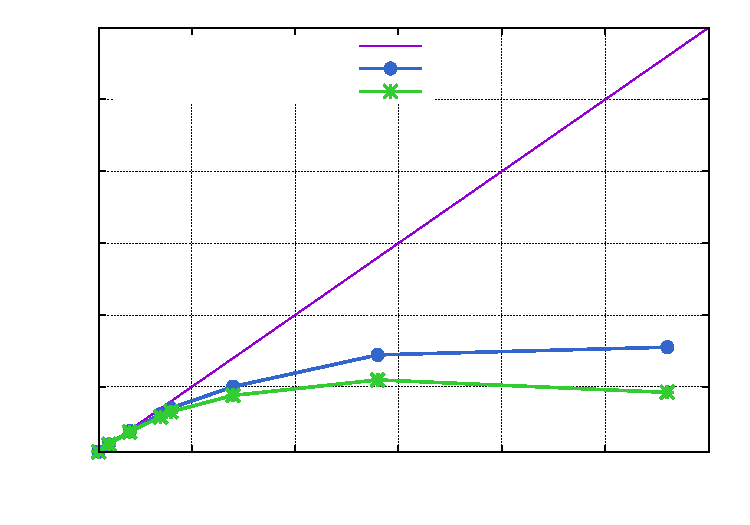
\includegraphics{plot-comp-T-s_nogatherInt_selected_500_4000_56_slide}}%
    \gplfronttext
  \end{picture}%
\endgroup
}
    \column{.5\columnwidth}
    \resizebox{\columnwidth}{!}{% GNUPLOT: LaTeX picture with Postscript
\begingroup
  \makeatletter
  \providecommand\color[2][]{%
    \GenericError{(gnuplot) \space\space\space\@spaces}{%
      Package color not loaded in conjunction with
      terminal option `colourtext'%
    }{See the gnuplot documentation for explanation.%
    }{Either use 'blacktext' in gnuplot or load the package
      color.sty in LaTeX.}%
    \renewcommand\color[2][]{}%
  }%
  \providecommand\includegraphics[2][]{%
    \GenericError{(gnuplot) \space\space\space\@spaces}{%
      Package graphicx or graphics not loaded%
    }{See the gnuplot documentation for explanation.%
    }{The gnuplot epslatex terminal needs graphicx.sty or graphics.sty.}%
    \renewcommand\includegraphics[2][]{}%
  }%
  \providecommand\rotatebox[2]{#2}%
  \@ifundefined{ifGPcolor}{%
    \newif\ifGPcolor
    \GPcolortrue
  }{}%
  \@ifundefined{ifGPblacktext}{%
    \newif\ifGPblacktext
    \GPblacktexttrue
  }{}%
  % define a \g@addto@macro without @ in the name:
  \let\gplgaddtomacro\g@addto@macro
  % define empty templates for all commands taking text:
  \gdef\gplbacktext{}%
  \gdef\gplfronttext{}%
  \makeatother
  \ifGPblacktext
    % no textcolor at all
    \def\colorrgb#1{}%
    \def\colorgray#1{}%
  \else
    % gray or color?
    \ifGPcolor
      \def\colorrgb#1{\color[rgb]{#1}}%
      \def\colorgray#1{\color[gray]{#1}}%
      \expandafter\def\csname LTw\endcsname{\color{white}}%
      \expandafter\def\csname LTb\endcsname{\color{black}}%
      \expandafter\def\csname LTa\endcsname{\color{black}}%
      \expandafter\def\csname LT0\endcsname{\color[rgb]{1,0,0}}%
      \expandafter\def\csname LT1\endcsname{\color[rgb]{0,1,0}}%
      \expandafter\def\csname LT2\endcsname{\color[rgb]{0,0,1}}%
      \expandafter\def\csname LT3\endcsname{\color[rgb]{1,0,1}}%
      \expandafter\def\csname LT4\endcsname{\color[rgb]{0,1,1}}%
      \expandafter\def\csname LT5\endcsname{\color[rgb]{1,1,0}}%
      \expandafter\def\csname LT6\endcsname{\color[rgb]{0,0,0}}%
      \expandafter\def\csname LT7\endcsname{\color[rgb]{1,0.3,0}}%
      \expandafter\def\csname LT8\endcsname{\color[rgb]{0.5,0.5,0.5}}%
    \else
      % gray
      \def\colorrgb#1{\color{black}}%
      \def\colorgray#1{\color[gray]{#1}}%
      \expandafter\def\csname LTw\endcsname{\color{white}}%
      \expandafter\def\csname LTb\endcsname{\color{black}}%
      \expandafter\def\csname LTa\endcsname{\color{black}}%
      \expandafter\def\csname LT0\endcsname{\color{black}}%
      \expandafter\def\csname LT1\endcsname{\color{black}}%
      \expandafter\def\csname LT2\endcsname{\color{black}}%
      \expandafter\def\csname LT3\endcsname{\color{black}}%
      \expandafter\def\csname LT4\endcsname{\color{black}}%
      \expandafter\def\csname LT5\endcsname{\color{black}}%
      \expandafter\def\csname LT6\endcsname{\color{black}}%
      \expandafter\def\csname LT7\endcsname{\color{black}}%
      \expandafter\def\csname LT8\endcsname{\color{black}}%
    \fi
  \fi
  \setlength{\unitlength}{0.0500bp}%
  \begin{picture}(7200.00,5040.00)%
    \gplgaddtomacro\gplbacktext{%
      \csname LTb\endcsname%
      \put(946,704){\makebox(0,0)[r]{\strut{} 1}}%
      \csname LTb\endcsname%
      \put(946,2740){\makebox(0,0)[r]{\strut{} 10}}%
      \csname LTb\endcsname%
      \put(946,4775){\makebox(0,0)[r]{\strut{} 100}}%
      \csname LTb\endcsname%
      \put(1951,484){\makebox(0,0){\strut{} 10}}%
      \csname LTb\endcsname%
      \put(2922,484){\makebox(0,0){\strut{} 20}}%
      \csname LTb\endcsname%
      \put(3892,484){\makebox(0,0){\strut{} 30}}%
      \csname LTb\endcsname%
      \put(4862,484){\makebox(0,0){\strut{} 40}}%
      \csname LTb\endcsname%
      \put(5833,484){\makebox(0,0){\strut{} 50}}%
      \csname LTb\endcsname%
      \put(6803,484){\makebox(0,0){\strut{} 60}}%
      \put(176,2739){\rotatebox{-270}{\makebox(0,0){\strut{}service time ($\,\mu\mathrm{sec}$\,)}}}%
      \put(3940,154){\makebox(0,0){\strut{}$n$ parallel degree}}%
    }%
    \gplgaddtomacro\gplfronttext{%
      \csname LTb\endcsname%
      \put(3586,4602){\makebox(0,0)[r]{\strut{}ideal service time}}%
      \csname LTb\endcsname%
      \put(3586,4382){\makebox(0,0)[r]{\strut{}udn udn}}%
      \csname LTb\endcsname%
      \put(3586,4162){\makebox(0,0)[r]{\strut{}sm sm}}%
    }%
    \gplbacktext
    \put(0,0){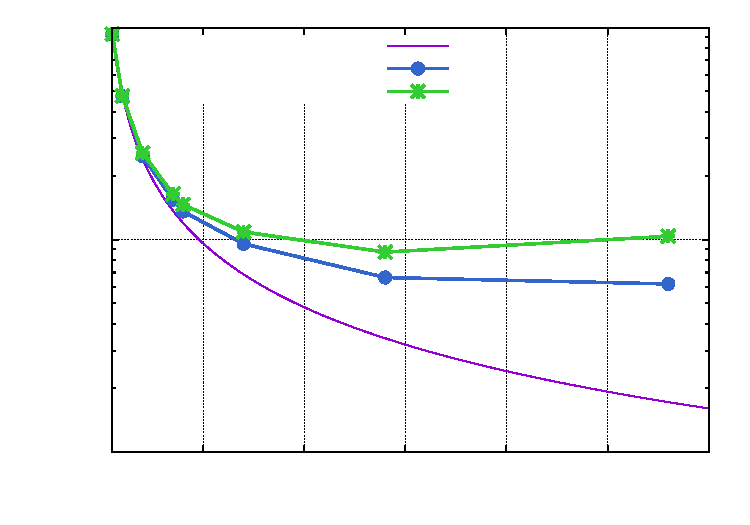
\includegraphics{plot-T-UDN-SM_nogatherInt_selected_500_selected_56_slide}}%
    \gplfronttext
  \end{picture}%
\endgroup
}
  \end{columns}
\end{frame}

\begin{frame}
  \frametitle{Confronto: tempo di servizio (2)}
  \begin{itemize}
  \item Tempo di interarrivo 4.627 \musec %23.133 \musec
  \item Dimensione delle matrici 168x168
  \item Tempo di servizio migliore UDN 25.092 \musec
  \item Tempo di servizio migliore SM 27.810 \musec  
  \end{itemize}
  \begin{columns}
    \column{.5\columnwidth}
    \resizebox{\columnwidth}{!}{% GNUPLOT: LaTeX picture with Postscript
\begingroup
  \makeatletter
  \providecommand\color[2][]{%
    \GenericError{(gnuplot) \space\space\space\@spaces}{%
      Package color not loaded in conjunction with
      terminal option `colourtext'%
    }{See the gnuplot documentation for explanation.%
    }{Either use 'blacktext' in gnuplot or load the package
      color.sty in LaTeX.}%
    \renewcommand\color[2][]{}%
  }%
  \providecommand\includegraphics[2][]{%
    \GenericError{(gnuplot) \space\space\space\@spaces}{%
      Package graphicx or graphics not loaded%
    }{See the gnuplot documentation for explanation.%
    }{The gnuplot epslatex terminal needs graphicx.sty or graphics.sty.}%
    \renewcommand\includegraphics[2][]{}%
  }%
  \providecommand\rotatebox[2]{#2}%
  \@ifundefined{ifGPcolor}{%
    \newif\ifGPcolor
    \GPcolortrue
  }{}%
  \@ifundefined{ifGPblacktext}{%
    \newif\ifGPblacktext
    \GPblacktexttrue
  }{}%
  % define a \g@addto@macro without @ in the name:
  \let\gplgaddtomacro\g@addto@macro
  % define empty templates for all commands taking text:
  \gdef\gplbacktext{}%
  \gdef\gplfronttext{}%
  \makeatother
  \ifGPblacktext
    % no textcolor at all
    \def\colorrgb#1{}%
    \def\colorgray#1{}%
  \else
    % gray or color?
    \ifGPcolor
      \def\colorrgb#1{\color[rgb]{#1}}%
      \def\colorgray#1{\color[gray]{#1}}%
      \expandafter\def\csname LTw\endcsname{\color{white}}%
      \expandafter\def\csname LTb\endcsname{\color{black}}%
      \expandafter\def\csname LTa\endcsname{\color{black}}%
      \expandafter\def\csname LT0\endcsname{\color[rgb]{1,0,0}}%
      \expandafter\def\csname LT1\endcsname{\color[rgb]{0,1,0}}%
      \expandafter\def\csname LT2\endcsname{\color[rgb]{0,0,1}}%
      \expandafter\def\csname LT3\endcsname{\color[rgb]{1,0,1}}%
      \expandafter\def\csname LT4\endcsname{\color[rgb]{0,1,1}}%
      \expandafter\def\csname LT5\endcsname{\color[rgb]{1,1,0}}%
      \expandafter\def\csname LT6\endcsname{\color[rgb]{0,0,0}}%
      \expandafter\def\csname LT7\endcsname{\color[rgb]{1,0.3,0}}%
      \expandafter\def\csname LT8\endcsname{\color[rgb]{0.5,0.5,0.5}}%
    \else
      % gray
      \def\colorrgb#1{\color{black}}%
      \def\colorgray#1{\color[gray]{#1}}%
      \expandafter\def\csname LTw\endcsname{\color{white}}%
      \expandafter\def\csname LTb\endcsname{\color{black}}%
      \expandafter\def\csname LTa\endcsname{\color{black}}%
      \expandafter\def\csname LT0\endcsname{\color{black}}%
      \expandafter\def\csname LT1\endcsname{\color{black}}%
      \expandafter\def\csname LT2\endcsname{\color{black}}%
      \expandafter\def\csname LT3\endcsname{\color{black}}%
      \expandafter\def\csname LT4\endcsname{\color{black}}%
      \expandafter\def\csname LT5\endcsname{\color{black}}%
      \expandafter\def\csname LT6\endcsname{\color{black}}%
      \expandafter\def\csname LT7\endcsname{\color{black}}%
      \expandafter\def\csname LT8\endcsname{\color{black}}%
    \fi
  \fi
  \setlength{\unitlength}{0.0500bp}%
  \begin{picture}(7200.00,5040.00)%
    \gplgaddtomacro\gplbacktext{%
      \csname LTb\endcsname%
      \put(814,1325){\makebox(0,0)[r]{\strut{} 10}}%
      \csname LTb\endcsname%
      \put(814,2015){\makebox(0,0)[r]{\strut{} 20}}%
      \csname LTb\endcsname%
      \put(814,2705){\makebox(0,0)[r]{\strut{} 30}}%
      \csname LTb\endcsname%
      \put(814,3395){\makebox(0,0)[r]{\strut{} 40}}%
      \csname LTb\endcsname%
      \put(814,4085){\makebox(0,0)[r]{\strut{} 50}}%
      \csname LTb\endcsname%
      \put(814,4775){\makebox(0,0)[r]{\strut{} 60}}%
      \csname LTb\endcsname%
      \put(1839,484){\makebox(0,0){\strut{} 10}}%
      \csname LTb\endcsname%
      \put(2832,484){\makebox(0,0){\strut{} 20}}%
      \csname LTb\endcsname%
      \put(3825,484){\makebox(0,0){\strut{} 30}}%
      \csname LTb\endcsname%
      \put(4818,484){\makebox(0,0){\strut{} 40}}%
      \csname LTb\endcsname%
      \put(5810,484){\makebox(0,0){\strut{} 50}}%
      \csname LTb\endcsname%
      \put(6803,484){\makebox(0,0){\strut{} 60}}%
      \put(176,2739){\rotatebox{-270}{\makebox(0,0){\strut{}scalability}}}%
      \put(3874,154){\makebox(0,0){\strut{}$n$ parallel degree}}%
    }%
    \gplgaddtomacro\gplfronttext{%
      \csname LTb\endcsname%
      \put(3322,4602){\makebox(0,0)[r]{\strut{}ideal scalability}}%
      \csname LTb\endcsname%
      \put(3322,4382){\makebox(0,0)[r]{\strut{}udn udn}}%
      \csname LTb\endcsname%
      \put(3322,4162){\makebox(0,0)[r]{\strut{}sm sm}}%
    }%
    \gplbacktext
    \put(0,0){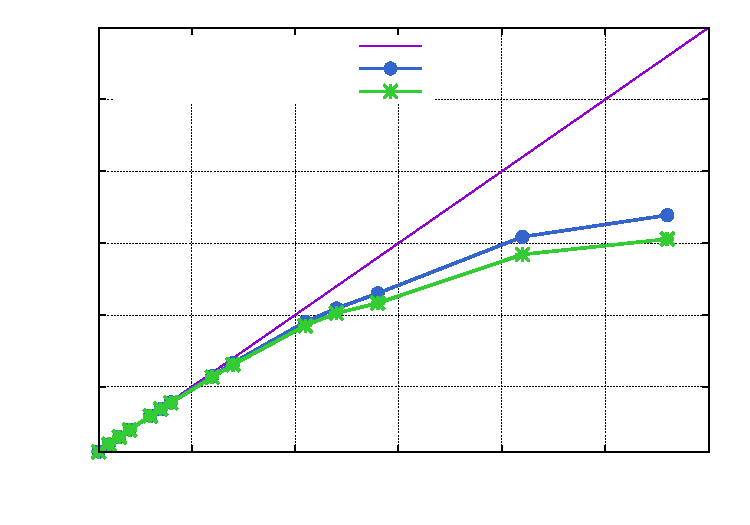
\includegraphics{plot-comp-T-s_nogatherInt_selected_500_20000_168_slide}}%
    \gplfronttext
  \end{picture}%
\endgroup
}
    \column{.5\columnwidth}
    \resizebox{\columnwidth}{!}{% GNUPLOT: LaTeX picture with Postscript
\begingroup
  \makeatletter
  \providecommand\color[2][]{%
    \GenericError{(gnuplot) \space\space\space\@spaces}{%
      Package color not loaded in conjunction with
      terminal option `colourtext'%
    }{See the gnuplot documentation for explanation.%
    }{Either use 'blacktext' in gnuplot or load the package
      color.sty in LaTeX.}%
    \renewcommand\color[2][]{}%
  }%
  \providecommand\includegraphics[2][]{%
    \GenericError{(gnuplot) \space\space\space\@spaces}{%
      Package graphicx or graphics not loaded%
    }{See the gnuplot documentation for explanation.%
    }{The gnuplot epslatex terminal needs graphicx.sty or graphics.sty.}%
    \renewcommand\includegraphics[2][]{}%
  }%
  \providecommand\rotatebox[2]{#2}%
  \@ifundefined{ifGPcolor}{%
    \newif\ifGPcolor
    \GPcolortrue
  }{}%
  \@ifundefined{ifGPblacktext}{%
    \newif\ifGPblacktext
    \GPblacktexttrue
  }{}%
  % define a \g@addto@macro without @ in the name:
  \let\gplgaddtomacro\g@addto@macro
  % define empty templates for all commands taking text:
  \gdef\gplbacktext{}%
  \gdef\gplfronttext{}%
  \makeatother
  \ifGPblacktext
    % no textcolor at all
    \def\colorrgb#1{}%
    \def\colorgray#1{}%
  \else
    % gray or color?
    \ifGPcolor
      \def\colorrgb#1{\color[rgb]{#1}}%
      \def\colorgray#1{\color[gray]{#1}}%
      \expandafter\def\csname LTw\endcsname{\color{white}}%
      \expandafter\def\csname LTb\endcsname{\color{black}}%
      \expandafter\def\csname LTa\endcsname{\color{black}}%
      \expandafter\def\csname LT0\endcsname{\color[rgb]{1,0,0}}%
      \expandafter\def\csname LT1\endcsname{\color[rgb]{0,1,0}}%
      \expandafter\def\csname LT2\endcsname{\color[rgb]{0,0,1}}%
      \expandafter\def\csname LT3\endcsname{\color[rgb]{1,0,1}}%
      \expandafter\def\csname LT4\endcsname{\color[rgb]{0,1,1}}%
      \expandafter\def\csname LT5\endcsname{\color[rgb]{1,1,0}}%
      \expandafter\def\csname LT6\endcsname{\color[rgb]{0,0,0}}%
      \expandafter\def\csname LT7\endcsname{\color[rgb]{1,0.3,0}}%
      \expandafter\def\csname LT8\endcsname{\color[rgb]{0.5,0.5,0.5}}%
    \else
      % gray
      \def\colorrgb#1{\color{black}}%
      \def\colorgray#1{\color[gray]{#1}}%
      \expandafter\def\csname LTw\endcsname{\color{white}}%
      \expandafter\def\csname LTb\endcsname{\color{black}}%
      \expandafter\def\csname LTa\endcsname{\color{black}}%
      \expandafter\def\csname LT0\endcsname{\color{black}}%
      \expandafter\def\csname LT1\endcsname{\color{black}}%
      \expandafter\def\csname LT2\endcsname{\color{black}}%
      \expandafter\def\csname LT3\endcsname{\color{black}}%
      \expandafter\def\csname LT4\endcsname{\color{black}}%
      \expandafter\def\csname LT5\endcsname{\color{black}}%
      \expandafter\def\csname LT6\endcsname{\color{black}}%
      \expandafter\def\csname LT7\endcsname{\color{black}}%
      \expandafter\def\csname LT8\endcsname{\color{black}}%
    \fi
  \fi
  \setlength{\unitlength}{0.0500bp}%
  \begin{picture}(7200.00,5040.00)%
    \gplgaddtomacro\gplbacktext{%
      \csname LTb\endcsname%
      \put(1078,704){\makebox(0,0)[r]{\strut{} 10}}%
      \csname LTb\endcsname%
      \put(1078,2740){\makebox(0,0)[r]{\strut{} 100}}%
      \csname LTb\endcsname%
      \put(1078,4775){\makebox(0,0)[r]{\strut{} 1000}}%
      \csname LTb\endcsname%
      \put(2063,484){\makebox(0,0){\strut{} 10}}%
      \csname LTb\endcsname%
      \put(3011,484){\makebox(0,0){\strut{} 20}}%
      \csname LTb\endcsname%
      \put(3959,484){\makebox(0,0){\strut{} 30}}%
      \csname LTb\endcsname%
      \put(4907,484){\makebox(0,0){\strut{} 40}}%
      \csname LTb\endcsname%
      \put(5855,484){\makebox(0,0){\strut{} 50}}%
      \csname LTb\endcsname%
      \put(6803,484){\makebox(0,0){\strut{} 60}}%
      \put(176,2739){\rotatebox{-270}{\makebox(0,0){\strut{}service time ($\,\mu\mathrm{sec}$\,)}}}%
      \put(4006,154){\makebox(0,0){\strut{}$n$ parallel degree}}%
    }%
    \gplgaddtomacro\gplfronttext{%
      \csname LTb\endcsname%
      \put(3718,4602){\makebox(0,0)[r]{\strut{}ideal service time}}%
      \csname LTb\endcsname%
      \put(3718,4382){\makebox(0,0)[r]{\strut{}udn udn}}%
      \csname LTb\endcsname%
      \put(3718,4162){\makebox(0,0)[r]{\strut{}sm sm}}%
    }%
    \gplbacktext
    \put(0,0){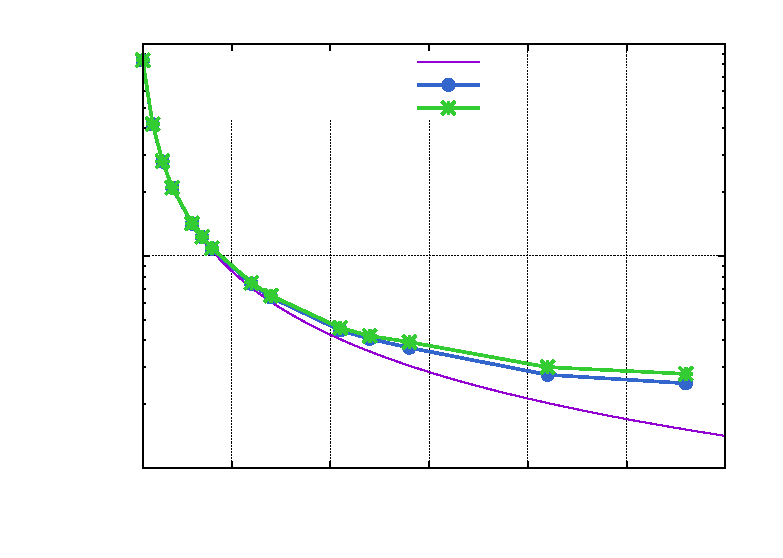
\includegraphics{plot-T-UDN-SM_nogatherInt_selected_500_selected_168_slide}}%
    \gplfronttext
  \end{picture}%
\endgroup
}
  \end{columns}
\end{frame}

\begin{frame}
  \frametitle{Confronto: tempo di servizio (3)}
  \begin{itemize}
  \item Tempo di interarrivo 4.627 \musec %57.831 \musec
  \item Dimensione delle matrici 280x280
  \item Tempo di servizio migliore UDN 62.943 \musec
  \item Tempo di servizio migliore SM 63.893 \musec  
  \end{itemize}
  \begin{columns}
    \column{.5\columnwidth}
    \resizebox{\columnwidth}{!}{% GNUPLOT: LaTeX picture with Postscript
\begingroup
  \makeatletter
  \providecommand\color[2][]{%
    \GenericError{(gnuplot) \space\space\space\@spaces}{%
      Package color not loaded in conjunction with
      terminal option `colourtext'%
    }{See the gnuplot documentation for explanation.%
    }{Either use 'blacktext' in gnuplot or load the package
      color.sty in LaTeX.}%
    \renewcommand\color[2][]{}%
  }%
  \providecommand\includegraphics[2][]{%
    \GenericError{(gnuplot) \space\space\space\@spaces}{%
      Package graphicx or graphics not loaded%
    }{See the gnuplot documentation for explanation.%
    }{The gnuplot epslatex terminal needs graphicx.sty or graphics.sty.}%
    \renewcommand\includegraphics[2][]{}%
  }%
  \providecommand\rotatebox[2]{#2}%
  \@ifundefined{ifGPcolor}{%
    \newif\ifGPcolor
    \GPcolortrue
  }{}%
  \@ifundefined{ifGPblacktext}{%
    \newif\ifGPblacktext
    \GPblacktexttrue
  }{}%
  % define a \g@addto@macro without @ in the name:
  \let\gplgaddtomacro\g@addto@macro
  % define empty templates for all commands taking text:
  \gdef\gplbacktext{}%
  \gdef\gplfronttext{}%
  \makeatother
  \ifGPblacktext
    % no textcolor at all
    \def\colorrgb#1{}%
    \def\colorgray#1{}%
  \else
    % gray or color?
    \ifGPcolor
      \def\colorrgb#1{\color[rgb]{#1}}%
      \def\colorgray#1{\color[gray]{#1}}%
      \expandafter\def\csname LTw\endcsname{\color{white}}%
      \expandafter\def\csname LTb\endcsname{\color{black}}%
      \expandafter\def\csname LTa\endcsname{\color{black}}%
      \expandafter\def\csname LT0\endcsname{\color[rgb]{1,0,0}}%
      \expandafter\def\csname LT1\endcsname{\color[rgb]{0,1,0}}%
      \expandafter\def\csname LT2\endcsname{\color[rgb]{0,0,1}}%
      \expandafter\def\csname LT3\endcsname{\color[rgb]{1,0,1}}%
      \expandafter\def\csname LT4\endcsname{\color[rgb]{0,1,1}}%
      \expandafter\def\csname LT5\endcsname{\color[rgb]{1,1,0}}%
      \expandafter\def\csname LT6\endcsname{\color[rgb]{0,0,0}}%
      \expandafter\def\csname LT7\endcsname{\color[rgb]{1,0.3,0}}%
      \expandafter\def\csname LT8\endcsname{\color[rgb]{0.5,0.5,0.5}}%
    \else
      % gray
      \def\colorrgb#1{\color{black}}%
      \def\colorgray#1{\color[gray]{#1}}%
      \expandafter\def\csname LTw\endcsname{\color{white}}%
      \expandafter\def\csname LTb\endcsname{\color{black}}%
      \expandafter\def\csname LTa\endcsname{\color{black}}%
      \expandafter\def\csname LT0\endcsname{\color{black}}%
      \expandafter\def\csname LT1\endcsname{\color{black}}%
      \expandafter\def\csname LT2\endcsname{\color{black}}%
      \expandafter\def\csname LT3\endcsname{\color{black}}%
      \expandafter\def\csname LT4\endcsname{\color{black}}%
      \expandafter\def\csname LT5\endcsname{\color{black}}%
      \expandafter\def\csname LT6\endcsname{\color{black}}%
      \expandafter\def\csname LT7\endcsname{\color{black}}%
      \expandafter\def\csname LT8\endcsname{\color{black}}%
    \fi
  \fi
  \setlength{\unitlength}{0.0500bp}%
  \begin{picture}(7200.00,5040.00)%
    \gplgaddtomacro\gplbacktext{%
      \csname LTb\endcsname%
      \put(814,1325){\makebox(0,0)[r]{\strut{} 10}}%
      \csname LTb\endcsname%
      \put(814,2015){\makebox(0,0)[r]{\strut{} 20}}%
      \csname LTb\endcsname%
      \put(814,2705){\makebox(0,0)[r]{\strut{} 30}}%
      \csname LTb\endcsname%
      \put(814,3395){\makebox(0,0)[r]{\strut{} 40}}%
      \csname LTb\endcsname%
      \put(814,4085){\makebox(0,0)[r]{\strut{} 50}}%
      \csname LTb\endcsname%
      \put(814,4775){\makebox(0,0)[r]{\strut{} 60}}%
      \csname LTb\endcsname%
      \put(1839,484){\makebox(0,0){\strut{} 10}}%
      \csname LTb\endcsname%
      \put(2832,484){\makebox(0,0){\strut{} 20}}%
      \csname LTb\endcsname%
      \put(3825,484){\makebox(0,0){\strut{} 30}}%
      \csname LTb\endcsname%
      \put(4818,484){\makebox(0,0){\strut{} 40}}%
      \csname LTb\endcsname%
      \put(5810,484){\makebox(0,0){\strut{} 50}}%
      \csname LTb\endcsname%
      \put(6803,484){\makebox(0,0){\strut{} 60}}%
      \put(176,2739){\rotatebox{-270}{\makebox(0,0){\strut{}scalability}}}%
      \put(3874,154){\makebox(0,0){\strut{}$n$ parallel degree}}%
    }%
    \gplgaddtomacro\gplfronttext{%
      \csname LTb\endcsname%
      \put(3322,4602){\makebox(0,0)[r]{\strut{}ideal scalability}}%
      \csname LTb\endcsname%
      \put(3322,4382){\makebox(0,0)[r]{\strut{}udn udn}}%
      \csname LTb\endcsname%
      \put(3322,4162){\makebox(0,0)[r]{\strut{}sm sm}}%
    }%
    \gplbacktext
    \put(0,0){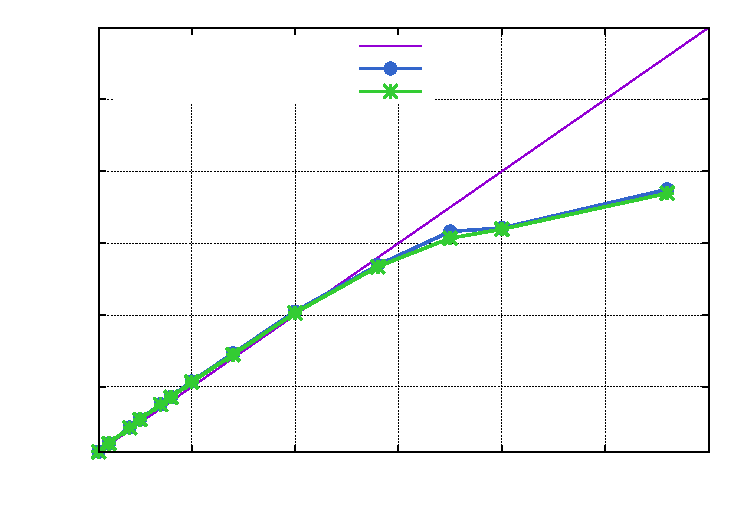
\includegraphics{plot-comp-T-s_nogatherInt_selected_500_50000_280_slide}}%
    \gplfronttext
  \end{picture}%
\endgroup
}
    \column{.5\columnwidth}
    \resizebox{\columnwidth}{!}{% GNUPLOT: LaTeX picture with Postscript
\begingroup
  \makeatletter
  \providecommand\color[2][]{%
    \GenericError{(gnuplot) \space\space\space\@spaces}{%
      Package color not loaded in conjunction with
      terminal option `colourtext'%
    }{See the gnuplot documentation for explanation.%
    }{Either use 'blacktext' in gnuplot or load the package
      color.sty in LaTeX.}%
    \renewcommand\color[2][]{}%
  }%
  \providecommand\includegraphics[2][]{%
    \GenericError{(gnuplot) \space\space\space\@spaces}{%
      Package graphicx or graphics not loaded%
    }{See the gnuplot documentation for explanation.%
    }{The gnuplot epslatex terminal needs graphicx.sty or graphics.sty.}%
    \renewcommand\includegraphics[2][]{}%
  }%
  \providecommand\rotatebox[2]{#2}%
  \@ifundefined{ifGPcolor}{%
    \newif\ifGPcolor
    \GPcolortrue
  }{}%
  \@ifundefined{ifGPblacktext}{%
    \newif\ifGPblacktext
    \GPblacktexttrue
  }{}%
  % define a \g@addto@macro without @ in the name:
  \let\gplgaddtomacro\g@addto@macro
  % define empty templates for all commands taking text:
  \gdef\gplbacktext{}%
  \gdef\gplfronttext{}%
  \makeatother
  \ifGPblacktext
    % no textcolor at all
    \def\colorrgb#1{}%
    \def\colorgray#1{}%
  \else
    % gray or color?
    \ifGPcolor
      \def\colorrgb#1{\color[rgb]{#1}}%
      \def\colorgray#1{\color[gray]{#1}}%
      \expandafter\def\csname LTw\endcsname{\color{white}}%
      \expandafter\def\csname LTb\endcsname{\color{black}}%
      \expandafter\def\csname LTa\endcsname{\color{black}}%
      \expandafter\def\csname LT0\endcsname{\color[rgb]{1,0,0}}%
      \expandafter\def\csname LT1\endcsname{\color[rgb]{0,1,0}}%
      \expandafter\def\csname LT2\endcsname{\color[rgb]{0,0,1}}%
      \expandafter\def\csname LT3\endcsname{\color[rgb]{1,0,1}}%
      \expandafter\def\csname LT4\endcsname{\color[rgb]{0,1,1}}%
      \expandafter\def\csname LT5\endcsname{\color[rgb]{1,1,0}}%
      \expandafter\def\csname LT6\endcsname{\color[rgb]{0,0,0}}%
      \expandafter\def\csname LT7\endcsname{\color[rgb]{1,0.3,0}}%
      \expandafter\def\csname LT8\endcsname{\color[rgb]{0.5,0.5,0.5}}%
    \else
      % gray
      \def\colorrgb#1{\color{black}}%
      \def\colorgray#1{\color[gray]{#1}}%
      \expandafter\def\csname LTw\endcsname{\color{white}}%
      \expandafter\def\csname LTb\endcsname{\color{black}}%
      \expandafter\def\csname LTa\endcsname{\color{black}}%
      \expandafter\def\csname LT0\endcsname{\color{black}}%
      \expandafter\def\csname LT1\endcsname{\color{black}}%
      \expandafter\def\csname LT2\endcsname{\color{black}}%
      \expandafter\def\csname LT3\endcsname{\color{black}}%
      \expandafter\def\csname LT4\endcsname{\color{black}}%
      \expandafter\def\csname LT5\endcsname{\color{black}}%
      \expandafter\def\csname LT6\endcsname{\color{black}}%
      \expandafter\def\csname LT7\endcsname{\color{black}}%
      \expandafter\def\csname LT8\endcsname{\color{black}}%
    \fi
  \fi
  \setlength{\unitlength}{0.0500bp}%
  \begin{picture}(7200.00,5040.00)%
    \gplgaddtomacro\gplbacktext{%
      \csname LTb\endcsname%
      \put(1210,704){\makebox(0,0)[r]{\strut{} 10}}%
      \csname LTb\endcsname%
      \put(1210,2061){\makebox(0,0)[r]{\strut{} 100}}%
      \csname LTb\endcsname%
      \put(1210,3418){\makebox(0,0)[r]{\strut{} 1000}}%
      \csname LTb\endcsname%
      \put(1210,4775){\makebox(0,0)[r]{\strut{} 10000}}%
      \csname LTb\endcsname%
      \put(2175,484){\makebox(0,0){\strut{} 10}}%
      \csname LTb\endcsname%
      \put(3101,484){\makebox(0,0){\strut{} 20}}%
      \csname LTb\endcsname%
      \put(4026,484){\makebox(0,0){\strut{} 30}}%
      \csname LTb\endcsname%
      \put(4952,484){\makebox(0,0){\strut{} 40}}%
      \csname LTb\endcsname%
      \put(5877,484){\makebox(0,0){\strut{} 50}}%
      \csname LTb\endcsname%
      \put(6803,484){\makebox(0,0){\strut{} 60}}%
      \put(176,2739){\rotatebox{-270}{\makebox(0,0){\strut{}service time ($\,\mu\mathrm{sec}$\,)}}}%
      \put(4072,154){\makebox(0,0){\strut{}$n$ parallel degree}}%
    }%
    \gplgaddtomacro\gplfronttext{%
      \csname LTb\endcsname%
      \put(3850,4602){\makebox(0,0)[r]{\strut{}ideal service time}}%
      \csname LTb\endcsname%
      \put(3850,4382){\makebox(0,0)[r]{\strut{}udn udn}}%
      \csname LTb\endcsname%
      \put(3850,4162){\makebox(0,0)[r]{\strut{}sm sm}}%
    }%
    \gplbacktext
    \put(0,0){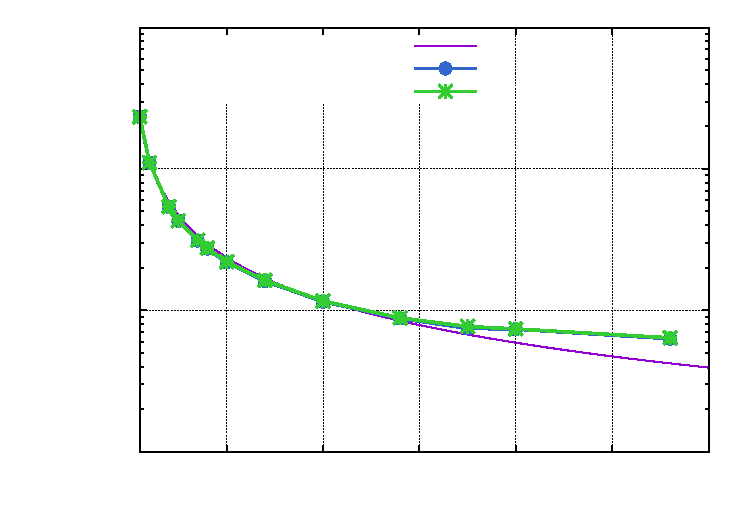
\includegraphics{plot-T-UDN-SM_nogatherInt_selected_500_selected_280_slide}}%
    \gplfronttext
  \end{picture}%
\endgroup
}
  \end{columns}
\end{frame}

\begin{frame}
  \frametitle{Confronto: tempo di servizio Multicast}
  \begin{columns}
    \column{.5\columnwidth}
    Dimensione delle matrici 56x56
    \column{.5\columnwidth}
    Dimensione delle matrici 280x280
  \end{columns}
  \vspace{5mm}
  \begin{columns}[c]
    \column{.5\columnwidth}
    \resizebox{\columnwidth}{!}{% GNUPLOT: LaTeX picture with Postscript
\begingroup
  \makeatletter
  \providecommand\color[2][]{%
    \GenericError{(gnuplot) \space\space\space\@spaces}{%
      Package color not loaded in conjunction with
      terminal option `colourtext'%
    }{See the gnuplot documentation for explanation.%
    }{Either use 'blacktext' in gnuplot or load the package
      color.sty in LaTeX.}%
    \renewcommand\color[2][]{}%
  }%
  \providecommand\includegraphics[2][]{%
    \GenericError{(gnuplot) \space\space\space\@spaces}{%
      Package graphicx or graphics not loaded%
    }{See the gnuplot documentation for explanation.%
    }{The gnuplot epslatex terminal needs graphicx.sty or graphics.sty.}%
    \renewcommand\includegraphics[2][]{}%
  }%
  \providecommand\rotatebox[2]{#2}%
  \@ifundefined{ifGPcolor}{%
    \newif\ifGPcolor
    \GPcolortrue
  }{}%
  \@ifundefined{ifGPblacktext}{%
    \newif\ifGPblacktext
    \GPblacktexttrue
  }{}%
  % define a \g@addto@macro without @ in the name:
  \let\gplgaddtomacro\g@addto@macro
  % define empty templates for all commands taking text:
  \gdef\gplbacktext{}%
  \gdef\gplfronttext{}%
  \makeatother
  \ifGPblacktext
    % no textcolor at all
    \def\colorrgb#1{}%
    \def\colorgray#1{}%
  \else
    % gray or color?
    \ifGPcolor
      \def\colorrgb#1{\color[rgb]{#1}}%
      \def\colorgray#1{\color[gray]{#1}}%
      \expandafter\def\csname LTw\endcsname{\color{white}}%
      \expandafter\def\csname LTb\endcsname{\color{black}}%
      \expandafter\def\csname LTa\endcsname{\color{black}}%
      \expandafter\def\csname LT0\endcsname{\color[rgb]{1,0,0}}%
      \expandafter\def\csname LT1\endcsname{\color[rgb]{0,1,0}}%
      \expandafter\def\csname LT2\endcsname{\color[rgb]{0,0,1}}%
      \expandafter\def\csname LT3\endcsname{\color[rgb]{1,0,1}}%
      \expandafter\def\csname LT4\endcsname{\color[rgb]{0,1,1}}%
      \expandafter\def\csname LT5\endcsname{\color[rgb]{1,1,0}}%
      \expandafter\def\csname LT6\endcsname{\color[rgb]{0,0,0}}%
      \expandafter\def\csname LT7\endcsname{\color[rgb]{1,0.3,0}}%
      \expandafter\def\csname LT8\endcsname{\color[rgb]{0.5,0.5,0.5}}%
    \else
      % gray
      \def\colorrgb#1{\color{black}}%
      \def\colorgray#1{\color[gray]{#1}}%
      \expandafter\def\csname LTw\endcsname{\color{white}}%
      \expandafter\def\csname LTb\endcsname{\color{black}}%
      \expandafter\def\csname LTa\endcsname{\color{black}}%
      \expandafter\def\csname LT0\endcsname{\color{black}}%
      \expandafter\def\csname LT1\endcsname{\color{black}}%
      \expandafter\def\csname LT2\endcsname{\color{black}}%
      \expandafter\def\csname LT3\endcsname{\color{black}}%
      \expandafter\def\csname LT4\endcsname{\color{black}}%
      \expandafter\def\csname LT5\endcsname{\color{black}}%
      \expandafter\def\csname LT6\endcsname{\color{black}}%
      \expandafter\def\csname LT7\endcsname{\color{black}}%
      \expandafter\def\csname LT8\endcsname{\color{black}}%
    \fi
  \fi
  \setlength{\unitlength}{0.0500bp}%
  \begin{picture}(7200.00,5040.00)%
    \gplgaddtomacro\gplbacktext{%
      \csname LTb\endcsname%
      \put(946,704){\makebox(0,0)[r]{\strut{} 0}}%
      \csname LTb\endcsname%
      \put(946,1629){\makebox(0,0)[r]{\strut{} 0.5}}%
      \csname LTb\endcsname%
      \put(946,2554){\makebox(0,0)[r]{\strut{} 1}}%
      \csname LTb\endcsname%
      \put(946,3480){\makebox(0,0)[r]{\strut{} 1.5}}%
      \csname LTb\endcsname%
      \put(946,4405){\makebox(0,0)[r]{\strut{} 2}}%
      \csname LTb\endcsname%
      \put(1951,484){\makebox(0,0){\strut{} 10}}%
      \csname LTb\endcsname%
      \put(2922,484){\makebox(0,0){\strut{} 20}}%
      \csname LTb\endcsname%
      \put(3892,484){\makebox(0,0){\strut{} 30}}%
      \csname LTb\endcsname%
      \put(4862,484){\makebox(0,0){\strut{} 40}}%
      \csname LTb\endcsname%
      \put(5833,484){\makebox(0,0){\strut{} 50}}%
      \csname LTb\endcsname%
      \put(6803,484){\makebox(0,0){\strut{} 60}}%
      \put(176,2739){\rotatebox{-270}{\makebox(0,0){\strut{}multicast service time $(\,\mu\textrm{sec}\,)$}}}%
      \put(3940,154){\makebox(0,0){\strut{}$n$ parallel degree}}%
    }%
    \gplgaddtomacro\gplfronttext{%
      \csname LTb\endcsname%
      \put(2134,4602){\makebox(0,0)[r]{\strut{}udn udn}}%
      \csname LTb\endcsname%
      \put(2134,4382){\makebox(0,0)[r]{\strut{}sm sm}}%
    }%
    \gplbacktext
    \put(0,0){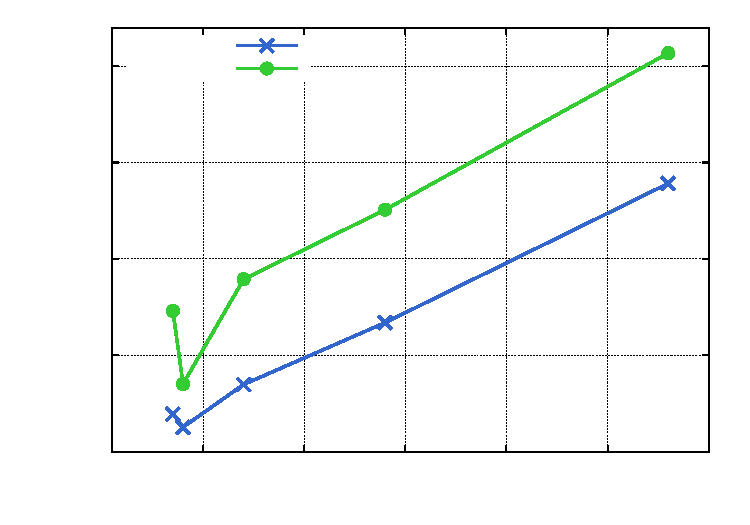
\includegraphics{plot-Tmult-UDN-SM-millis_nogatherInt_selected_500_selected_56_slide}}%
    \gplfronttext
  \end{picture}%
\endgroup
}
    \column{.5\columnwidth}
    \resizebox{\columnwidth}{!}{% GNUPLOT: LaTeX picture with Postscript
\begingroup
  \makeatletter
  \providecommand\color[2][]{%
    \GenericError{(gnuplot) \space\space\space\@spaces}{%
      Package color not loaded in conjunction with
      terminal option `colourtext'%
    }{See the gnuplot documentation for explanation.%
    }{Either use 'blacktext' in gnuplot or load the package
      color.sty in LaTeX.}%
    \renewcommand\color[2][]{}%
  }%
  \providecommand\includegraphics[2][]{%
    \GenericError{(gnuplot) \space\space\space\@spaces}{%
      Package graphicx or graphics not loaded%
    }{See the gnuplot documentation for explanation.%
    }{The gnuplot epslatex terminal needs graphicx.sty or graphics.sty.}%
    \renewcommand\includegraphics[2][]{}%
  }%
  \providecommand\rotatebox[2]{#2}%
  \@ifundefined{ifGPcolor}{%
    \newif\ifGPcolor
    \GPcolortrue
  }{}%
  \@ifundefined{ifGPblacktext}{%
    \newif\ifGPblacktext
    \GPblacktexttrue
  }{}%
  % define a \g@addto@macro without @ in the name:
  \let\gplgaddtomacro\g@addto@macro
  % define empty templates for all commands taking text:
  \gdef\gplbacktext{}%
  \gdef\gplfronttext{}%
  \makeatother
  \ifGPblacktext
    % no textcolor at all
    \def\colorrgb#1{}%
    \def\colorgray#1{}%
  \else
    % gray or color?
    \ifGPcolor
      \def\colorrgb#1{\color[rgb]{#1}}%
      \def\colorgray#1{\color[gray]{#1}}%
      \expandafter\def\csname LTw\endcsname{\color{white}}%
      \expandafter\def\csname LTb\endcsname{\color{black}}%
      \expandafter\def\csname LTa\endcsname{\color{black}}%
      \expandafter\def\csname LT0\endcsname{\color[rgb]{1,0,0}}%
      \expandafter\def\csname LT1\endcsname{\color[rgb]{0,1,0}}%
      \expandafter\def\csname LT2\endcsname{\color[rgb]{0,0,1}}%
      \expandafter\def\csname LT3\endcsname{\color[rgb]{1,0,1}}%
      \expandafter\def\csname LT4\endcsname{\color[rgb]{0,1,1}}%
      \expandafter\def\csname LT5\endcsname{\color[rgb]{1,1,0}}%
      \expandafter\def\csname LT6\endcsname{\color[rgb]{0,0,0}}%
      \expandafter\def\csname LT7\endcsname{\color[rgb]{1,0.3,0}}%
      \expandafter\def\csname LT8\endcsname{\color[rgb]{0.5,0.5,0.5}}%
    \else
      % gray
      \def\colorrgb#1{\color{black}}%
      \def\colorgray#1{\color[gray]{#1}}%
      \expandafter\def\csname LTw\endcsname{\color{white}}%
      \expandafter\def\csname LTb\endcsname{\color{black}}%
      \expandafter\def\csname LTa\endcsname{\color{black}}%
      \expandafter\def\csname LT0\endcsname{\color{black}}%
      \expandafter\def\csname LT1\endcsname{\color{black}}%
      \expandafter\def\csname LT2\endcsname{\color{black}}%
      \expandafter\def\csname LT3\endcsname{\color{black}}%
      \expandafter\def\csname LT4\endcsname{\color{black}}%
      \expandafter\def\csname LT5\endcsname{\color{black}}%
      \expandafter\def\csname LT6\endcsname{\color{black}}%
      \expandafter\def\csname LT7\endcsname{\color{black}}%
      \expandafter\def\csname LT8\endcsname{\color{black}}%
    \fi
  \fi
  \setlength{\unitlength}{0.0500bp}%
  \begin{picture}(7200.00,5040.00)%
    \gplgaddtomacro\gplbacktext{%
      \csname LTb\endcsname%
      \put(946,704){\makebox(0,0)[r]{\strut{} 0}}%
      \csname LTb\endcsname%
      \put(946,1629){\makebox(0,0)[r]{\strut{} 0.5}}%
      \csname LTb\endcsname%
      \put(946,2554){\makebox(0,0)[r]{\strut{} 1}}%
      \csname LTb\endcsname%
      \put(946,3480){\makebox(0,0)[r]{\strut{} 1.5}}%
      \csname LTb\endcsname%
      \put(946,4405){\makebox(0,0)[r]{\strut{} 2}}%
      \csname LTb\endcsname%
      \put(1951,484){\makebox(0,0){\strut{} 10}}%
      \csname LTb\endcsname%
      \put(2922,484){\makebox(0,0){\strut{} 20}}%
      \csname LTb\endcsname%
      \put(3892,484){\makebox(0,0){\strut{} 30}}%
      \csname LTb\endcsname%
      \put(4862,484){\makebox(0,0){\strut{} 40}}%
      \csname LTb\endcsname%
      \put(5833,484){\makebox(0,0){\strut{} 50}}%
      \csname LTb\endcsname%
      \put(6803,484){\makebox(0,0){\strut{} 60}}%
      \put(176,2739){\rotatebox{-270}{\makebox(0,0){\strut{}multicast service time $(\,\mu\textrm{sec}\,)$}}}%
      \put(3940,154){\makebox(0,0){\strut{}$n$ parallel degree}}%
    }%
    \gplgaddtomacro\gplfronttext{%
      \csname LTb\endcsname%
      \put(2134,4602){\makebox(0,0)[r]{\strut{}udn udn}}%
      \csname LTb\endcsname%
      \put(2134,4382){\makebox(0,0)[r]{\strut{}sm sm}}%
    }%
    \gplbacktext
    \put(0,0){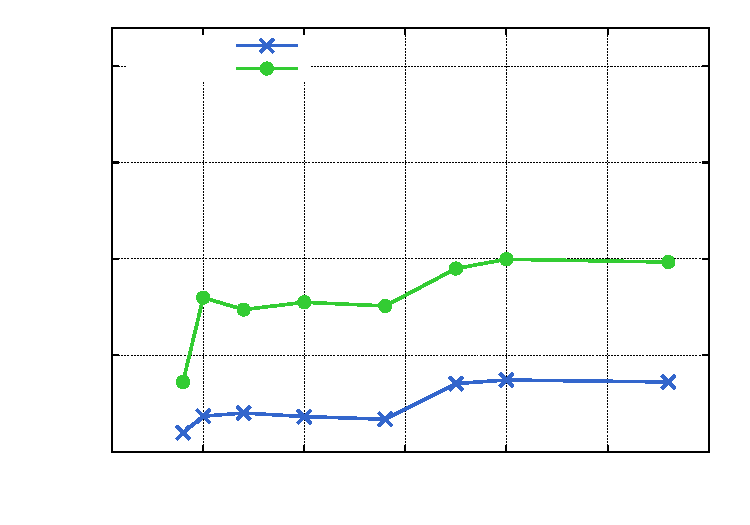
\includegraphics{plot-Tmult-UDN-SM-millis_nogatherInt_selected_500_selected_280_slide}}%
    \gplfronttext
  \end{picture}%
\endgroup
}
  \end{columns}  
\end{frame}

\begin{frame}
  \frametitle{Confronto: tempo di calcolo di un singolo prodotto scalare}
  \framesubtitle{Tipo di dato: 'Intero'}
  \begin{columns}[c]
    \column{.5\columnwidth}
    \resizebox{\columnwidth}{!}{% GNUPLOT: LaTeX picture with Postscript
\begingroup
  \makeatletter
  \providecommand\color[2][]{%
    \GenericError{(gnuplot) \space\space\space\@spaces}{%
      Package color not loaded in conjunction with
      terminal option `colourtext'%
    }{See the gnuplot documentation for explanation.%
    }{Either use 'blacktext' in gnuplot or load the package
      color.sty in LaTeX.}%
    \renewcommand\color[2][]{}%
  }%
  \providecommand\includegraphics[2][]{%
    \GenericError{(gnuplot) \space\space\space\@spaces}{%
      Package graphicx or graphics not loaded%
    }{See the gnuplot documentation for explanation.%
    }{The gnuplot epslatex terminal needs graphicx.sty or graphics.sty.}%
    \renewcommand\includegraphics[2][]{}%
  }%
  \providecommand\rotatebox[2]{#2}%
  \@ifundefined{ifGPcolor}{%
    \newif\ifGPcolor
    \GPcolortrue
  }{}%
  \@ifundefined{ifGPblacktext}{%
    \newif\ifGPblacktext
    \GPblacktextfalse
  }{}%
  % define a \g@addto@macro without @ in the name:
  \let\gplgaddtomacro\g@addto@macro
  % define empty templates for all commands taking text:
  \gdef\gplbacktext{}%
  \gdef\gplfronttext{}%
  \makeatother
  \ifGPblacktext
    % no textcolor at all
    \def\colorrgb#1{}%
    \def\colorgray#1{}%
  \else
    % gray or color?
    \ifGPcolor
      \def\colorrgb#1{\color[rgb]{#1}}%
      \def\colorgray#1{\color[gray]{#1}}%
      \expandafter\def\csname LTw\endcsname{\color{white}}%
      \expandafter\def\csname LTb\endcsname{\color{black}}%
      \expandafter\def\csname LTa\endcsname{\color{black}}%
      \expandafter\def\csname LT0\endcsname{\color[rgb]{1,0,0}}%
      \expandafter\def\csname LT1\endcsname{\color[rgb]{0,1,0}}%
      \expandafter\def\csname LT2\endcsname{\color[rgb]{0,0,1}}%
      \expandafter\def\csname LT3\endcsname{\color[rgb]{1,0,1}}%
      \expandafter\def\csname LT4\endcsname{\color[rgb]{0,1,1}}%
      \expandafter\def\csname LT5\endcsname{\color[rgb]{1,1,0}}%
      \expandafter\def\csname LT6\endcsname{\color[rgb]{0,0,0}}%
      \expandafter\def\csname LT7\endcsname{\color[rgb]{1,0.3,0}}%
      \expandafter\def\csname LT8\endcsname{\color[rgb]{0.5,0.5,0.5}}%
    \else
      % gray
      \def\colorrgb#1{\color{black}}%
      \def\colorgray#1{\color[gray]{#1}}%
      \expandafter\def\csname LTw\endcsname{\color{white}}%
      \expandafter\def\csname LTb\endcsname{\color{black}}%
      \expandafter\def\csname LTa\endcsname{\color{black}}%
      \expandafter\def\csname LT0\endcsname{\color{black}}%
      \expandafter\def\csname LT1\endcsname{\color{black}}%
      \expandafter\def\csname LT2\endcsname{\color{black}}%
      \expandafter\def\csname LT3\endcsname{\color{black}}%
      \expandafter\def\csname LT4\endcsname{\color{black}}%
      \expandafter\def\csname LT5\endcsname{\color{black}}%
      \expandafter\def\csname LT6\endcsname{\color{black}}%
      \expandafter\def\csname LT7\endcsname{\color{black}}%
      \expandafter\def\csname LT8\endcsname{\color{black}}%
    \fi
  \fi
  \setlength{\unitlength}{0.0500bp}%
  \begin{picture}(7200.00,5040.00)%
    \gplgaddtomacro\gplbacktext{%
      \csname LTb\endcsname%
      \put(946,1074){\makebox(0,0)[r]{\strut{} 1}}%
      \csname LTb\endcsname%
      \put(946,1999){\makebox(0,0)[r]{\strut{} 1.5}}%
      \csname LTb\endcsname%
      \put(946,2925){\makebox(0,0)[r]{\strut{} 2}}%
      \csname LTb\endcsname%
      \put(946,3850){\makebox(0,0)[r]{\strut{} 2.5}}%
      \csname LTb\endcsname%
      \put(946,4775){\makebox(0,0)[r]{\strut{} 3}}%
      \csname LTb\endcsname%
      \put(1951,484){\makebox(0,0){\strut{} 10}}%
      \csname LTb\endcsname%
      \put(2922,484){\makebox(0,0){\strut{} 20}}%
      \csname LTb\endcsname%
      \put(3892,484){\makebox(0,0){\strut{} 30}}%
      \csname LTb\endcsname%
      \put(4862,484){\makebox(0,0){\strut{} 40}}%
      \csname LTb\endcsname%
      \put(5833,484){\makebox(0,0){\strut{} 50}}%
      \csname LTb\endcsname%
      \put(6803,484){\makebox(0,0){\strut{} 60}}%
      \put(176,2739){\rotatebox{-270}{\makebox(0,0){\strut{}$T_{\textrm{row}}^{\phantom{row}(n)} / T_{\textrm{row}}^{\phantom{row}(1)}$}}}%
      \put(3940,154){\makebox(0,0){\strut{}$n$ parallel degree}}%
    }%
    \gplgaddtomacro\gplfronttext{%
      \csname LTb\endcsname%
      \put(3718,4602){\makebox(0,0)[r]{\strut{}Matrix Size 280x280}}%
      \csname LTb\endcsname%
      \put(3718,4382){\makebox(0,0)[r]{\strut{}Matrix Size 168x168}}%
      \csname LTb\endcsname%
      \put(3718,4162){\makebox(0,0)[r]{\strut{}Matrix Size 56x56}}%
    }%
    \gplbacktext
    \put(0,0){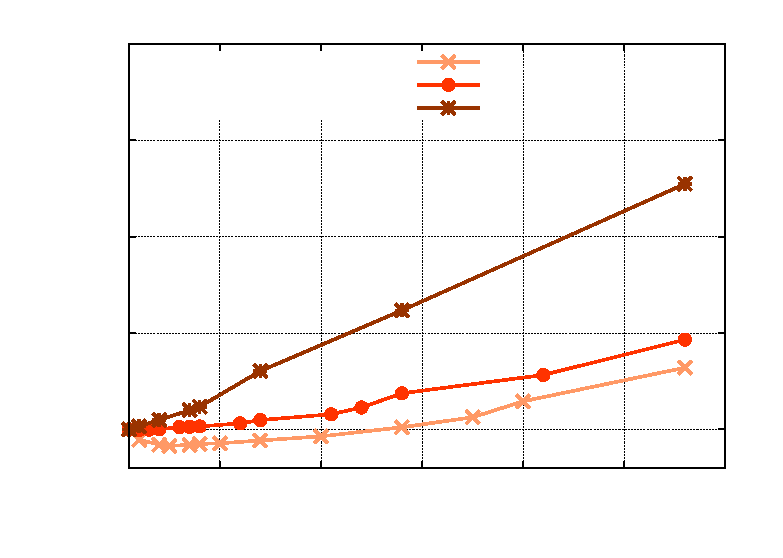
\includegraphics{plot-rowCalcT_nogatherInt_00_500_4000_all_slide}}%
    \gplfronttext
  \end{picture}%
\endgroup
}
    \column{.5\columnwidth}
    \resizebox{\columnwidth}{!}{% GNUPLOT: LaTeX picture with Postscript
\begingroup
  \makeatletter
  \providecommand\color[2][]{%
    \GenericError{(gnuplot) \space\space\space\@spaces}{%
      Package color not loaded in conjunction with
      terminal option `colourtext'%
    }{See the gnuplot documentation for explanation.%
    }{Either use 'blacktext' in gnuplot or load the package
      color.sty in LaTeX.}%
    \renewcommand\color[2][]{}%
  }%
  \providecommand\includegraphics[2][]{%
    \GenericError{(gnuplot) \space\space\space\@spaces}{%
      Package graphicx or graphics not loaded%
    }{See the gnuplot documentation for explanation.%
    }{The gnuplot epslatex terminal needs graphicx.sty or graphics.sty.}%
    \renewcommand\includegraphics[2][]{}%
  }%
  \providecommand\rotatebox[2]{#2}%
  \@ifundefined{ifGPcolor}{%
    \newif\ifGPcolor
    \GPcolortrue
  }{}%
  \@ifundefined{ifGPblacktext}{%
    \newif\ifGPblacktext
    \GPblacktextfalse
  }{}%
  % define a \g@addto@macro without @ in the name:
  \let\gplgaddtomacro\g@addto@macro
  % define empty templates for all commands taking text:
  \gdef\gplbacktext{}%
  \gdef\gplfronttext{}%
  \makeatother
  \ifGPblacktext
    % no textcolor at all
    \def\colorrgb#1{}%
    \def\colorgray#1{}%
  \else
    % gray or color?
    \ifGPcolor
      \def\colorrgb#1{\color[rgb]{#1}}%
      \def\colorgray#1{\color[gray]{#1}}%
      \expandafter\def\csname LTw\endcsname{\color{white}}%
      \expandafter\def\csname LTb\endcsname{\color{black}}%
      \expandafter\def\csname LTa\endcsname{\color{black}}%
      \expandafter\def\csname LT0\endcsname{\color[rgb]{1,0,0}}%
      \expandafter\def\csname LT1\endcsname{\color[rgb]{0,1,0}}%
      \expandafter\def\csname LT2\endcsname{\color[rgb]{0,0,1}}%
      \expandafter\def\csname LT3\endcsname{\color[rgb]{1,0,1}}%
      \expandafter\def\csname LT4\endcsname{\color[rgb]{0,1,1}}%
      \expandafter\def\csname LT5\endcsname{\color[rgb]{1,1,0}}%
      \expandafter\def\csname LT6\endcsname{\color[rgb]{0,0,0}}%
      \expandafter\def\csname LT7\endcsname{\color[rgb]{1,0.3,0}}%
      \expandafter\def\csname LT8\endcsname{\color[rgb]{0.5,0.5,0.5}}%
    \else
      % gray
      \def\colorrgb#1{\color{black}}%
      \def\colorgray#1{\color[gray]{#1}}%
      \expandafter\def\csname LTw\endcsname{\color{white}}%
      \expandafter\def\csname LTb\endcsname{\color{black}}%
      \expandafter\def\csname LTa\endcsname{\color{black}}%
      \expandafter\def\csname LT0\endcsname{\color{black}}%
      \expandafter\def\csname LT1\endcsname{\color{black}}%
      \expandafter\def\csname LT2\endcsname{\color{black}}%
      \expandafter\def\csname LT3\endcsname{\color{black}}%
      \expandafter\def\csname LT4\endcsname{\color{black}}%
      \expandafter\def\csname LT5\endcsname{\color{black}}%
      \expandafter\def\csname LT6\endcsname{\color{black}}%
      \expandafter\def\csname LT7\endcsname{\color{black}}%
      \expandafter\def\csname LT8\endcsname{\color{black}}%
    \fi
  \fi
  \setlength{\unitlength}{0.0500bp}%
  \begin{picture}(7200.00,5040.00)%
    \gplgaddtomacro\gplbacktext{%
      \csname LTb\endcsname%
      \put(946,1074){\makebox(0,0)[r]{\strut{} 1}}%
      \csname LTb\endcsname%
      \put(946,1999){\makebox(0,0)[r]{\strut{} 1.5}}%
      \csname LTb\endcsname%
      \put(946,2925){\makebox(0,0)[r]{\strut{} 2}}%
      \csname LTb\endcsname%
      \put(946,3850){\makebox(0,0)[r]{\strut{} 2.5}}%
      \csname LTb\endcsname%
      \put(946,4775){\makebox(0,0)[r]{\strut{} 3}}%
      \csname LTb\endcsname%
      \put(1951,484){\makebox(0,0){\strut{} 10}}%
      \csname LTb\endcsname%
      \put(2922,484){\makebox(0,0){\strut{} 20}}%
      \csname LTb\endcsname%
      \put(3892,484){\makebox(0,0){\strut{} 30}}%
      \csname LTb\endcsname%
      \put(4862,484){\makebox(0,0){\strut{} 40}}%
      \csname LTb\endcsname%
      \put(5833,484){\makebox(0,0){\strut{} 50}}%
      \csname LTb\endcsname%
      \put(6803,484){\makebox(0,0){\strut{} 60}}%
      \put(176,2739){\rotatebox{-270}{\makebox(0,0){\strut{}$T_{\textrm{row}}^{\phantom{row}(n)} / T_{\textrm{row}}^{\phantom{row}(1)}$}}}%
      \put(3940,154){\makebox(0,0){\strut{}$n$ parallel degree}}%
    }%
    \gplgaddtomacro\gplfronttext{%
      \csname LTb\endcsname%
      \put(3718,4602){\makebox(0,0)[r]{\strut{}Matrix Size 280x280}}%
      \csname LTb\endcsname%
      \put(3718,4382){\makebox(0,0)[r]{\strut{}Matrix Size 168x168}}%
      \csname LTb\endcsname%
      \put(3718,4162){\makebox(0,0)[r]{\strut{}Matrix Size 56x56}}%
    }%
    \gplbacktext
    \put(0,0){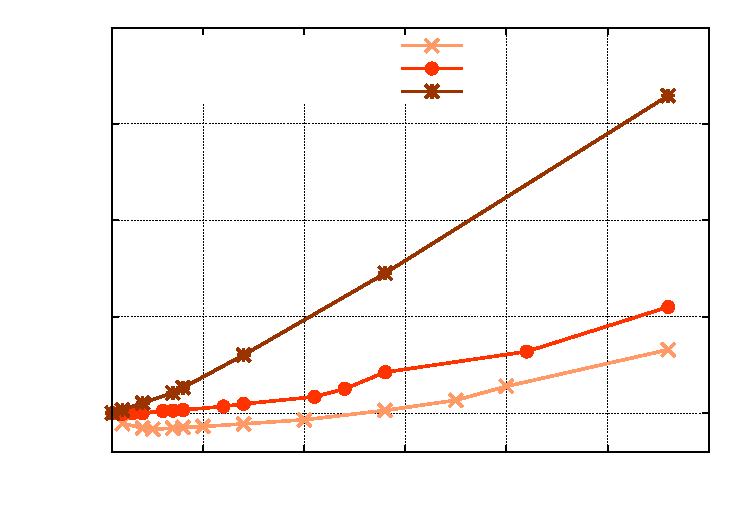
\includegraphics{plot-rowCalcT_nogatherInt_11_500_4000_all_slide}}%
    \gplfronttext
  \end{picture}%
\endgroup
}
  \end{columns} 
\end{frame}

\begin{frame}
  \frametitle{Confronto: tempo di calcolo di un singolo prodotto scalare}
  \framesubtitle{Tipo di dato: 'Virgola Mobile'}
  \begin{columns}[c]
    \column{.5\columnwidth}
    \resizebox{\columnwidth}{!}{% GNUPLOT: LaTeX picture with Postscript
\begingroup
  \makeatletter
  \providecommand\color[2][]{%
    \GenericError{(gnuplot) \space\space\space\@spaces}{%
      Package color not loaded in conjunction with
      terminal option `colourtext'%
    }{See the gnuplot documentation for explanation.%
    }{Either use 'blacktext' in gnuplot or load the package
      color.sty in LaTeX.}%
    \renewcommand\color[2][]{}%
  }%
  \providecommand\includegraphics[2][]{%
    \GenericError{(gnuplot) \space\space\space\@spaces}{%
      Package graphicx or graphics not loaded%
    }{See the gnuplot documentation for explanation.%
    }{The gnuplot epslatex terminal needs graphicx.sty or graphics.sty.}%
    \renewcommand\includegraphics[2][]{}%
  }%
  \providecommand\rotatebox[2]{#2}%
  \@ifundefined{ifGPcolor}{%
    \newif\ifGPcolor
    \GPcolortrue
  }{}%
  \@ifundefined{ifGPblacktext}{%
    \newif\ifGPblacktext
    \GPblacktextfalse
  }{}%
  % define a \g@addto@macro without @ in the name:
  \let\gplgaddtomacro\g@addto@macro
  % define empty templates for all commands taking text:
  \gdef\gplbacktext{}%
  \gdef\gplfronttext{}%
  \makeatother
  \ifGPblacktext
    % no textcolor at all
    \def\colorrgb#1{}%
    \def\colorgray#1{}%
  \else
    % gray or color?
    \ifGPcolor
      \def\colorrgb#1{\color[rgb]{#1}}%
      \def\colorgray#1{\color[gray]{#1}}%
      \expandafter\def\csname LTw\endcsname{\color{white}}%
      \expandafter\def\csname LTb\endcsname{\color{black}}%
      \expandafter\def\csname LTa\endcsname{\color{black}}%
      \expandafter\def\csname LT0\endcsname{\color[rgb]{1,0,0}}%
      \expandafter\def\csname LT1\endcsname{\color[rgb]{0,1,0}}%
      \expandafter\def\csname LT2\endcsname{\color[rgb]{0,0,1}}%
      \expandafter\def\csname LT3\endcsname{\color[rgb]{1,0,1}}%
      \expandafter\def\csname LT4\endcsname{\color[rgb]{0,1,1}}%
      \expandafter\def\csname LT5\endcsname{\color[rgb]{1,1,0}}%
      \expandafter\def\csname LT6\endcsname{\color[rgb]{0,0,0}}%
      \expandafter\def\csname LT7\endcsname{\color[rgb]{1,0.3,0}}%
      \expandafter\def\csname LT8\endcsname{\color[rgb]{0.5,0.5,0.5}}%
    \else
      % gray
      \def\colorrgb#1{\color{black}}%
      \def\colorgray#1{\color[gray]{#1}}%
      \expandafter\def\csname LTw\endcsname{\color{white}}%
      \expandafter\def\csname LTb\endcsname{\color{black}}%
      \expandafter\def\csname LTa\endcsname{\color{black}}%
      \expandafter\def\csname LT0\endcsname{\color{black}}%
      \expandafter\def\csname LT1\endcsname{\color{black}}%
      \expandafter\def\csname LT2\endcsname{\color{black}}%
      \expandafter\def\csname LT3\endcsname{\color{black}}%
      \expandafter\def\csname LT4\endcsname{\color{black}}%
      \expandafter\def\csname LT5\endcsname{\color{black}}%
      \expandafter\def\csname LT6\endcsname{\color{black}}%
      \expandafter\def\csname LT7\endcsname{\color{black}}%
      \expandafter\def\csname LT8\endcsname{\color{black}}%
    \fi
  \fi
  \setlength{\unitlength}{0.0500bp}%
  \begin{picture}(7200.00,5040.00)%
    \gplgaddtomacro\gplbacktext{%
      \csname LTb\endcsname%
      \put(946,1074){\makebox(0,0)[r]{\strut{} 1}}%
      \csname LTb\endcsname%
      \put(946,1999){\makebox(0,0)[r]{\strut{} 1.5}}%
      \csname LTb\endcsname%
      \put(946,2925){\makebox(0,0)[r]{\strut{} 2}}%
      \csname LTb\endcsname%
      \put(946,3850){\makebox(0,0)[r]{\strut{} 2.5}}%
      \csname LTb\endcsname%
      \put(946,4775){\makebox(0,0)[r]{\strut{} 3}}%
      \csname LTb\endcsname%
      \put(1951,484){\makebox(0,0){\strut{} 10}}%
      \csname LTb\endcsname%
      \put(2922,484){\makebox(0,0){\strut{} 20}}%
      \csname LTb\endcsname%
      \put(3892,484){\makebox(0,0){\strut{} 30}}%
      \csname LTb\endcsname%
      \put(4862,484){\makebox(0,0){\strut{} 40}}%
      \csname LTb\endcsname%
      \put(5833,484){\makebox(0,0){\strut{} 50}}%
      \csname LTb\endcsname%
      \put(6803,484){\makebox(0,0){\strut{} 60}}%
      \put(176,2739){\rotatebox{-270}{\makebox(0,0){\strut{}$T_{\textrm{row}}^{\phantom{row}(n)} / T_{\textrm{row}}^{\phantom{row}(1)}$}}}%
      \put(3940,154){\makebox(0,0){\strut{}$n$ parallel degree}}%
    }%
    \gplgaddtomacro\gplfronttext{%
      \csname LTb\endcsname%
      \put(3718,4602){\makebox(0,0)[r]{\strut{}Matrix Size 280x280}}%
      \csname LTb\endcsname%
      \put(3718,4382){\makebox(0,0)[r]{\strut{}Matrix Size 168x168}}%
      \csname LTb\endcsname%
      \put(3718,4162){\makebox(0,0)[r]{\strut{}Matrix Size 56x56}}%
    }%
    \gplbacktext
    \put(0,0){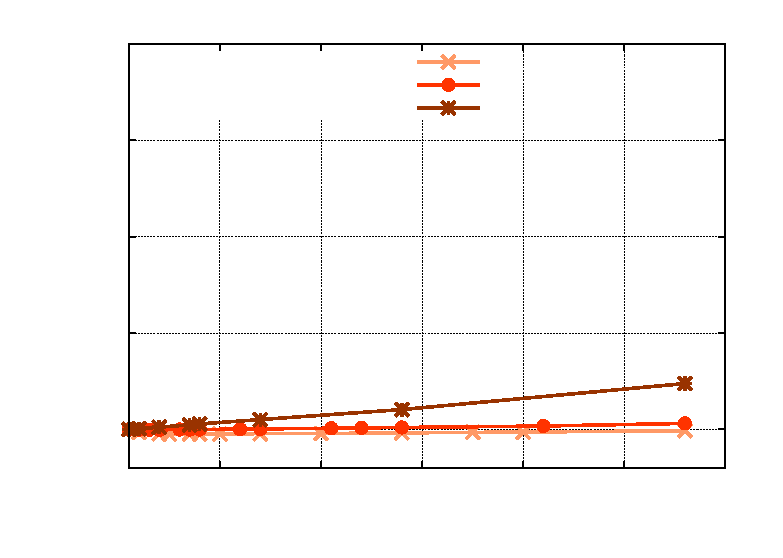
\includegraphics{plot-rowCalcT_nogatherFloat_00_500_4000_all_slide}}%
    \gplfronttext
  \end{picture}%
\endgroup
}
    \column{.5\columnwidth}
    \resizebox{\columnwidth}{!}{% GNUPLOT: LaTeX picture with Postscript
\begingroup
  \makeatletter
  \providecommand\color[2][]{%
    \GenericError{(gnuplot) \space\space\space\@spaces}{%
      Package color not loaded in conjunction with
      terminal option `colourtext'%
    }{See the gnuplot documentation for explanation.%
    }{Either use 'blacktext' in gnuplot or load the package
      color.sty in LaTeX.}%
    \renewcommand\color[2][]{}%
  }%
  \providecommand\includegraphics[2][]{%
    \GenericError{(gnuplot) \space\space\space\@spaces}{%
      Package graphicx or graphics not loaded%
    }{See the gnuplot documentation for explanation.%
    }{The gnuplot epslatex terminal needs graphicx.sty or graphics.sty.}%
    \renewcommand\includegraphics[2][]{}%
  }%
  \providecommand\rotatebox[2]{#2}%
  \@ifundefined{ifGPcolor}{%
    \newif\ifGPcolor
    \GPcolortrue
  }{}%
  \@ifundefined{ifGPblacktext}{%
    \newif\ifGPblacktext
    \GPblacktextfalse
  }{}%
  % define a \g@addto@macro without @ in the name:
  \let\gplgaddtomacro\g@addto@macro
  % define empty templates for all commands taking text:
  \gdef\gplbacktext{}%
  \gdef\gplfronttext{}%
  \makeatother
  \ifGPblacktext
    % no textcolor at all
    \def\colorrgb#1{}%
    \def\colorgray#1{}%
  \else
    % gray or color?
    \ifGPcolor
      \def\colorrgb#1{\color[rgb]{#1}}%
      \def\colorgray#1{\color[gray]{#1}}%
      \expandafter\def\csname LTw\endcsname{\color{white}}%
      \expandafter\def\csname LTb\endcsname{\color{black}}%
      \expandafter\def\csname LTa\endcsname{\color{black}}%
      \expandafter\def\csname LT0\endcsname{\color[rgb]{1,0,0}}%
      \expandafter\def\csname LT1\endcsname{\color[rgb]{0,1,0}}%
      \expandafter\def\csname LT2\endcsname{\color[rgb]{0,0,1}}%
      \expandafter\def\csname LT3\endcsname{\color[rgb]{1,0,1}}%
      \expandafter\def\csname LT4\endcsname{\color[rgb]{0,1,1}}%
      \expandafter\def\csname LT5\endcsname{\color[rgb]{1,1,0}}%
      \expandafter\def\csname LT6\endcsname{\color[rgb]{0,0,0}}%
      \expandafter\def\csname LT7\endcsname{\color[rgb]{1,0.3,0}}%
      \expandafter\def\csname LT8\endcsname{\color[rgb]{0.5,0.5,0.5}}%
    \else
      % gray
      \def\colorrgb#1{\color{black}}%
      \def\colorgray#1{\color[gray]{#1}}%
      \expandafter\def\csname LTw\endcsname{\color{white}}%
      \expandafter\def\csname LTb\endcsname{\color{black}}%
      \expandafter\def\csname LTa\endcsname{\color{black}}%
      \expandafter\def\csname LT0\endcsname{\color{black}}%
      \expandafter\def\csname LT1\endcsname{\color{black}}%
      \expandafter\def\csname LT2\endcsname{\color{black}}%
      \expandafter\def\csname LT3\endcsname{\color{black}}%
      \expandafter\def\csname LT4\endcsname{\color{black}}%
      \expandafter\def\csname LT5\endcsname{\color{black}}%
      \expandafter\def\csname LT6\endcsname{\color{black}}%
      \expandafter\def\csname LT7\endcsname{\color{black}}%
      \expandafter\def\csname LT8\endcsname{\color{black}}%
    \fi
  \fi
  \setlength{\unitlength}{0.0500bp}%
  \begin{picture}(7200.00,5040.00)%
    \gplgaddtomacro\gplbacktext{%
      \csname LTb\endcsname%
      \put(946,1074){\makebox(0,0)[r]{\strut{} 1}}%
      \csname LTb\endcsname%
      \put(946,1999){\makebox(0,0)[r]{\strut{} 1.5}}%
      \csname LTb\endcsname%
      \put(946,2925){\makebox(0,0)[r]{\strut{} 2}}%
      \csname LTb\endcsname%
      \put(946,3850){\makebox(0,0)[r]{\strut{} 2.5}}%
      \csname LTb\endcsname%
      \put(946,4775){\makebox(0,0)[r]{\strut{} 3}}%
      \csname LTb\endcsname%
      \put(1951,484){\makebox(0,0){\strut{} 10}}%
      \csname LTb\endcsname%
      \put(2922,484){\makebox(0,0){\strut{} 20}}%
      \csname LTb\endcsname%
      \put(3892,484){\makebox(0,0){\strut{} 30}}%
      \csname LTb\endcsname%
      \put(4862,484){\makebox(0,0){\strut{} 40}}%
      \csname LTb\endcsname%
      \put(5833,484){\makebox(0,0){\strut{} 50}}%
      \csname LTb\endcsname%
      \put(6803,484){\makebox(0,0){\strut{} 60}}%
      \put(176,2739){\rotatebox{-270}{\makebox(0,0){\strut{}$T_{\textrm{row}}^{\phantom{row}(n)} / T_{\textrm{row}}^{\phantom{row}(1)}$}}}%
      \put(3940,154){\makebox(0,0){\strut{}$n$ parallel degree}}%
    }%
    \gplgaddtomacro\gplfronttext{%
      \csname LTb\endcsname%
      \put(3718,4602){\makebox(0,0)[r]{\strut{}Matrix Size 280x280}}%
      \csname LTb\endcsname%
      \put(3718,4382){\makebox(0,0)[r]{\strut{}Matrix Size 168x168}}%
      \csname LTb\endcsname%
      \put(3718,4162){\makebox(0,0)[r]{\strut{}Matrix Size 56x56}}%
    }%
    \gplbacktext
    \put(0,0){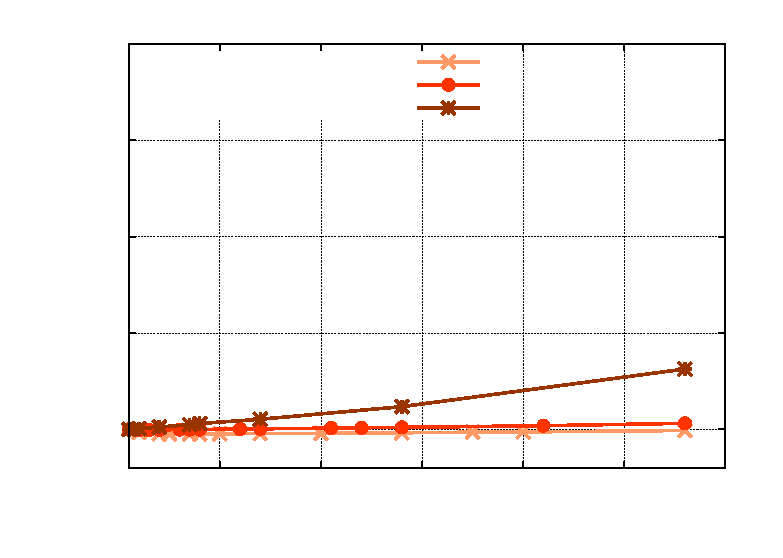
\includegraphics{plot-rowCalcT_nogatherFloat_11_500_4000_all_slide}}%
    \gplfronttext
  \end{picture}%
\endgroup
}
  \end{columns} 
\end{frame}

\end{document}

